% Options for packages loaded elsewhere
\PassOptionsToPackage{unicode}{hyperref}
\PassOptionsToPackage{hyphens}{url}
\PassOptionsToPackage{dvipsnames,svgnames,x11names}{xcolor}
%
\documentclass[
  letterpaper,
  DIV=11,
  numbers=noendperiod]{scrartcl}

\usepackage{amsmath,amssymb}
\usepackage{iftex}
\ifPDFTeX
  \usepackage[T1]{fontenc}
  \usepackage[utf8]{inputenc}
  \usepackage{textcomp} % provide euro and other symbols
\else % if luatex or xetex
  \usepackage{unicode-math}
  \defaultfontfeatures{Scale=MatchLowercase}
  \defaultfontfeatures[\rmfamily]{Ligatures=TeX,Scale=1}
\fi
\usepackage{lmodern}
\ifPDFTeX\else  
    % xetex/luatex font selection
\fi
% Use upquote if available, for straight quotes in verbatim environments
\IfFileExists{upquote.sty}{\usepackage{upquote}}{}
\IfFileExists{microtype.sty}{% use microtype if available
  \usepackage[]{microtype}
  \UseMicrotypeSet[protrusion]{basicmath} % disable protrusion for tt fonts
}{}
\makeatletter
\@ifundefined{KOMAClassName}{% if non-KOMA class
  \IfFileExists{parskip.sty}{%
    \usepackage{parskip}
  }{% else
    \setlength{\parindent}{0pt}
    \setlength{\parskip}{6pt plus 2pt minus 1pt}}
}{% if KOMA class
  \KOMAoptions{parskip=half}}
\makeatother
\usepackage{xcolor}
\setlength{\emergencystretch}{3em} % prevent overfull lines
\setcounter{secnumdepth}{-\maxdimen} % remove section numbering
% Make \paragraph and \subparagraph free-standing
\ifx\paragraph\undefined\else
  \let\oldparagraph\paragraph
  \renewcommand{\paragraph}[1]{\oldparagraph{#1}\mbox{}}
\fi
\ifx\subparagraph\undefined\else
  \let\oldsubparagraph\subparagraph
  \renewcommand{\subparagraph}[1]{\oldsubparagraph{#1}\mbox{}}
\fi

\usepackage{color}
\usepackage{fancyvrb}
\newcommand{\VerbBar}{|}
\newcommand{\VERB}{\Verb[commandchars=\\\{\}]}
\DefineVerbatimEnvironment{Highlighting}{Verbatim}{commandchars=\\\{\}}
% Add ',fontsize=\small' for more characters per line
\newenvironment{Shaded}{}{}
\newcommand{\AlertTok}[1]{\textcolor[rgb]{1.00,0.33,0.33}{\textbf{#1}}}
\newcommand{\AnnotationTok}[1]{\textcolor[rgb]{0.42,0.45,0.49}{#1}}
\newcommand{\AttributeTok}[1]{\textcolor[rgb]{0.84,0.23,0.29}{#1}}
\newcommand{\BaseNTok}[1]{\textcolor[rgb]{0.00,0.36,0.77}{#1}}
\newcommand{\BuiltInTok}[1]{\textcolor[rgb]{0.84,0.23,0.29}{#1}}
\newcommand{\CharTok}[1]{\textcolor[rgb]{0.01,0.18,0.38}{#1}}
\newcommand{\CommentTok}[1]{\textcolor[rgb]{0.42,0.45,0.49}{#1}}
\newcommand{\CommentVarTok}[1]{\textcolor[rgb]{0.42,0.45,0.49}{#1}}
\newcommand{\ConstantTok}[1]{\textcolor[rgb]{0.00,0.36,0.77}{#1}}
\newcommand{\ControlFlowTok}[1]{\textcolor[rgb]{0.84,0.23,0.29}{#1}}
\newcommand{\DataTypeTok}[1]{\textcolor[rgb]{0.84,0.23,0.29}{#1}}
\newcommand{\DecValTok}[1]{\textcolor[rgb]{0.00,0.36,0.77}{#1}}
\newcommand{\DocumentationTok}[1]{\textcolor[rgb]{0.42,0.45,0.49}{#1}}
\newcommand{\ErrorTok}[1]{\textcolor[rgb]{1.00,0.33,0.33}{\underline{#1}}}
\newcommand{\ExtensionTok}[1]{\textcolor[rgb]{0.84,0.23,0.29}{\textbf{#1}}}
\newcommand{\FloatTok}[1]{\textcolor[rgb]{0.00,0.36,0.77}{#1}}
\newcommand{\FunctionTok}[1]{\textcolor[rgb]{0.44,0.26,0.76}{#1}}
\newcommand{\ImportTok}[1]{\textcolor[rgb]{0.01,0.18,0.38}{#1}}
\newcommand{\InformationTok}[1]{\textcolor[rgb]{0.42,0.45,0.49}{#1}}
\newcommand{\KeywordTok}[1]{\textcolor[rgb]{0.84,0.23,0.29}{#1}}
\newcommand{\NormalTok}[1]{\textcolor[rgb]{0.14,0.16,0.18}{#1}}
\newcommand{\OperatorTok}[1]{\textcolor[rgb]{0.14,0.16,0.18}{#1}}
\newcommand{\OtherTok}[1]{\textcolor[rgb]{0.44,0.26,0.76}{#1}}
\newcommand{\PreprocessorTok}[1]{\textcolor[rgb]{0.84,0.23,0.29}{#1}}
\newcommand{\RegionMarkerTok}[1]{\textcolor[rgb]{0.42,0.45,0.49}{#1}}
\newcommand{\SpecialCharTok}[1]{\textcolor[rgb]{0.00,0.36,0.77}{#1}}
\newcommand{\SpecialStringTok}[1]{\textcolor[rgb]{0.01,0.18,0.38}{#1}}
\newcommand{\StringTok}[1]{\textcolor[rgb]{0.01,0.18,0.38}{#1}}
\newcommand{\VariableTok}[1]{\textcolor[rgb]{0.89,0.38,0.04}{#1}}
\newcommand{\VerbatimStringTok}[1]{\textcolor[rgb]{0.01,0.18,0.38}{#1}}
\newcommand{\WarningTok}[1]{\textcolor[rgb]{1.00,0.33,0.33}{#1}}

\providecommand{\tightlist}{%
  \setlength{\itemsep}{0pt}\setlength{\parskip}{0pt}}\usepackage{longtable,booktabs,array}
\usepackage{calc} % for calculating minipage widths
% Correct order of tables after \paragraph or \subparagraph
\usepackage{etoolbox}
\makeatletter
\patchcmd\longtable{\par}{\if@noskipsec\mbox{}\fi\par}{}{}
\makeatother
% Allow footnotes in longtable head/foot
\IfFileExists{footnotehyper.sty}{\usepackage{footnotehyper}}{\usepackage{footnote}}
\makesavenoteenv{longtable}
\usepackage{graphicx}
\makeatletter
\def\maxwidth{\ifdim\Gin@nat@width>\linewidth\linewidth\else\Gin@nat@width\fi}
\def\maxheight{\ifdim\Gin@nat@height>\textheight\textheight\else\Gin@nat@height\fi}
\makeatother
% Scale images if necessary, so that they will not overflow the page
% margins by default, and it is still possible to overwrite the defaults
% using explicit options in \includegraphics[width, height, ...]{}
\setkeys{Gin}{width=\maxwidth,height=\maxheight,keepaspectratio}
% Set default figure placement to htbp
\makeatletter
\def\fps@figure{htbp}
\makeatother

\KOMAoption{captions}{tableheading,figureheading}
\makeatletter
\makeatother
\makeatletter
\makeatother
\makeatletter
\@ifpackageloaded{caption}{}{\usepackage{caption}}
\AtBeginDocument{%
\ifdefined\contentsname
  \renewcommand*\contentsname{Tabla de contenidos}
\else
  \newcommand\contentsname{Tabla de contenidos}
\fi
\ifdefined\listfigurename
  \renewcommand*\listfigurename{Listado de Figuras}
\else
  \newcommand\listfigurename{Listado de Figuras}
\fi
\ifdefined\listtablename
  \renewcommand*\listtablename{Listado de Tablas}
\else
  \newcommand\listtablename{Listado de Tablas}
\fi
\ifdefined\figurename
  \renewcommand*\figurename{Figura}
\else
  \newcommand\figurename{Figura}
\fi
\ifdefined\tablename
  \renewcommand*\tablename{Tabla}
\else
  \newcommand\tablename{Tabla}
\fi
}
\@ifpackageloaded{float}{}{\usepackage{float}}
\floatstyle{ruled}
\@ifundefined{c@chapter}{\newfloat{codelisting}{h}{lop}}{\newfloat{codelisting}{h}{lop}[chapter]}
\floatname{codelisting}{Listado}
\newcommand*\listoflistings{\listof{codelisting}{Listado de Listados}}
\makeatother
\makeatletter
\@ifpackageloaded{caption}{}{\usepackage{caption}}
\@ifpackageloaded{subcaption}{}{\usepackage{subcaption}}
\makeatother
\makeatletter
\@ifpackageloaded{tcolorbox}{}{\usepackage[skins,breakable]{tcolorbox}}
\makeatother
\makeatletter
\@ifundefined{shadecolor}{\definecolor{shadecolor}{rgb}{.97, .97, .97}}
\makeatother
\makeatletter
\makeatother
\makeatletter
\makeatother
\ifLuaTeX
\usepackage[bidi=basic]{babel}
\else
\usepackage[bidi=default]{babel}
\fi
\babelprovide[main,import]{spanish}
% get rid of language-specific shorthands (see #6817):
\let\LanguageShortHands\languageshorthands
\def\languageshorthands#1{}
\ifLuaTeX
  \usepackage{selnolig}  % disable illegal ligatures
\fi
\usepackage[]{biblatex}
\addbibresource{../../../../references.bib}
\IfFileExists{bookmark.sty}{\usepackage{bookmark}}{\usepackage{hyperref}}
\IfFileExists{xurl.sty}{\usepackage{xurl}}{} % add URL line breaks if available
\urlstyle{same} % disable monospaced font for URLs
\hypersetup{
  pdftitle={¿Qué nos ofrece R?},
  pdfauthor={Edison Achalma},
  pdflang={es},
  colorlinks=true,
  linkcolor={blue},
  filecolor={Maroon},
  citecolor={Blue},
  urlcolor={Blue},
  pdfcreator={LaTeX via pandoc}}

\title{¿Qué nos ofrece R?}
\usepackage{etoolbox}
\makeatletter
\providecommand{\subtitle}[1]{% add subtitle to \maketitle
  \apptocmd{\@title}{\par {\large #1 \par}}{}{}
}
\makeatother
\subtitle{Explorando las capacidades de R y su uso en el entorno Linux}
\author{Edison Achalma}
\date{2023-06-10}

\begin{document}
\maketitle
\ifdefined\Shaded\renewenvironment{Shaded}{\begin{tcolorbox}[frame hidden, enhanced, boxrule=0pt, breakable, sharp corners, interior hidden, borderline west={3pt}{0pt}{shadecolor}]}{\end{tcolorbox}}\fi

\hypertarget{quxfae-nos-ofrece-rstudio}{%
\section{¿Qúe nos ofrece RStudio?}\label{quxfae-nos-ofrece-rstudio}}

\hypertarget{beneficios-del-software-rstudio}{%
\subsection{Beneficios del software
RStudio}\label{beneficios-del-software-rstudio}}

RStudio es una herramienta poderosa que brinda numerosas ventajas para
los usuarios. A continuación, destacamos algunas de las funcionalidades
que ofrece:

\begin{enumerate}
\def\labelenumi{\arabic{enumi}.}
\item
  \textbf{Potente editor de código:} RStudio proporciona un entorno de
  desarrollo integrado (IDE) que cuenta con un editor de código robusto.
  Este editor permite escribir, editar y ejecutar código de manera
  eficiente, lo que facilita el trabajo con el lenguaje de programación
  R.
\item
  \textbf{Gestión del espacio de trabajo:} RStudio ofrece
  características avanzadas para el manejo del espacio de trabajo.
  Puedes explorar y administrar fácilmente los objetos, variables y
  funciones utilizados en tu sesión de R, lo que facilita el seguimiento
  y la organización de tus datos y resultados.
\item
  \textbf{Depuración y resaltado de sintaxis:} La función de depuración
  de RStudio te permite identificar y corregir errores en tu código de
  manera eficiente. Además, el resaltado de sintaxis te ayuda a
  visualizar y comprender mejor la estructura de tu código, lo que
  facilita su lectura y mantenimiento.
\item
  \textbf{Autocompletado inteligente:} RStudio ofrece una función de
  autocompletado inteligente, que te sugiere opciones de código a medida
  que escribes. Esto acelera el proceso de codificación al proporcionar
  sugerencias contextuales y facilitar la escritura correcta de las
  funciones y objetos de R.
\item
  \textbf{Interoperabilidad con otros software y plataformas:} RStudio
  es compatible con una amplia gama de herramientas y plataformas.
  Puedes integrar fácilmente tus análisis en flujos de trabajo
  existentes, colaborar con otros profesionales y compartir tus
  resultados en diferentes formatos, como informes, gráficos
  interactivos o aplicaciones web.
\end{enumerate}

\begin{figure}

\caption{Interfaz de RStudio: Una poderosa herramienta para el
desarrollo en R}

{\centering 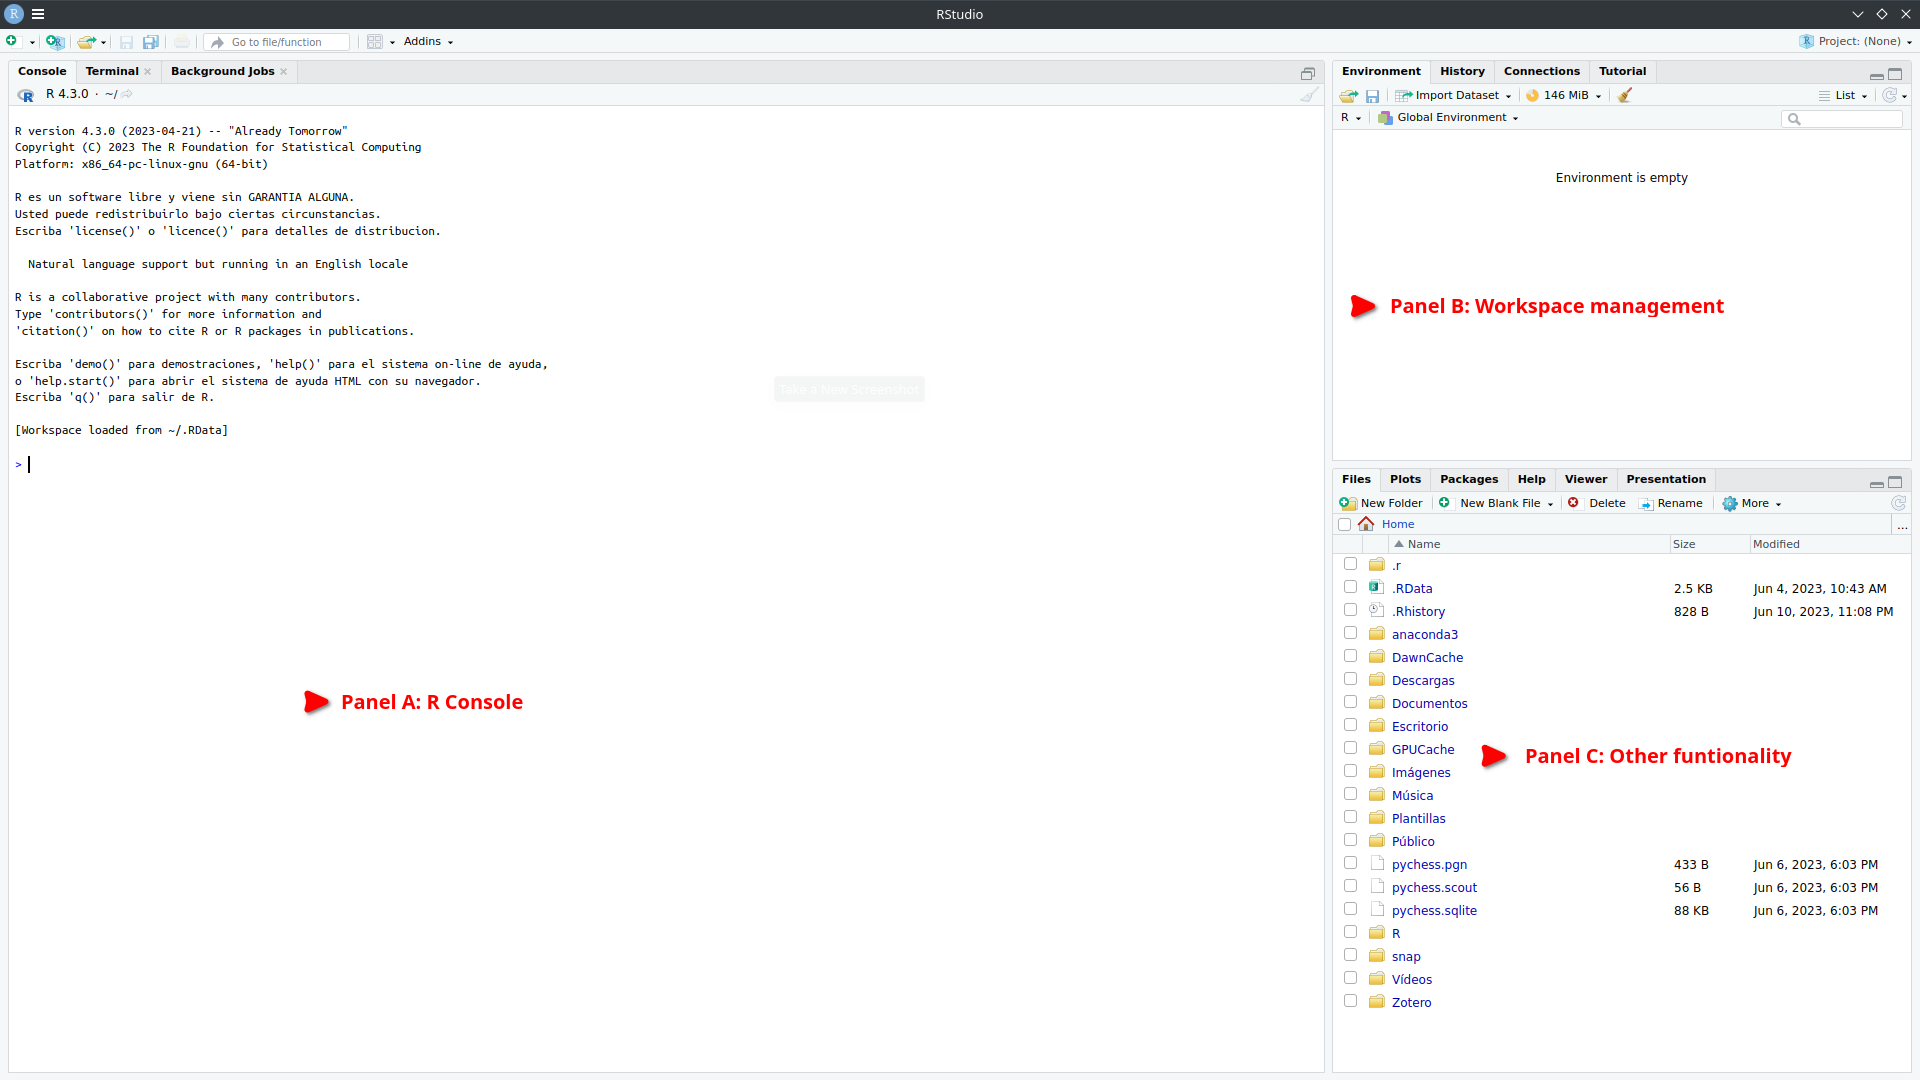
\includegraphics{images/Screenshot_20230610_233058.png}

}

\end{figure}

\hypertarget{archivos-de-script-en-r-.r}{%
\subsection{Archivos de Script en R
(.R)}\label{archivos-de-script-en-r-.r}}

En el mundo del análisis de datos y programación en R, los archivos de
script (.R) desempeñan un papel fundamental. Estos archivos contienen la
secuencia de comandos necesaria para realizar análisis y manipulación de
datos de manera sistemática y reproducible.

\hypertarget{ventajas-de-utilizar-archivos-de-script-en-r}{%
\subsubsection{Ventajas de utilizar archivos de script en
R:}\label{ventajas-de-utilizar-archivos-de-script-en-r}}

\begin{enumerate}
\def\labelenumi{\arabic{enumi}.}
\item
  \textbf{Documentación de tareas}: Al escribir nuestros comandos en un
  archivo de script, estamos creando una documentación detallada de los
  pasos y procesos utilizados en nuestro análisis. Esto facilita la
  comprensión y revisión de nuestro trabajo, tanto para nosotros mismos
  como para otros colaboradores.
\item
  \textbf{Automatización de tareas repetitivas}: Los archivos de script
  permiten automatizar tareas que se repiten con frecuencia. Podemos
  definir una serie de comandos en el archivo y ejecutarlos de forma
  rápida y eficiente cada vez que sea necesario. Esto ahorra tiempo y
  reduce la posibilidad de errores.
\item
  \textbf{Evaluación de cambios}: Al tener nuestros comandos en un
  archivo de script, podemos realizar modificaciones y ajustes en el
  análisis de manera más ágil. Podemos realizar pruebas y evaluaciones
  de los cambios sin necesidad de volver a escribir todo el código desde
  cero. Esto nos brinda flexibilidad y nos permite iterar y mejorar
  nuestro análisis de manera más eficiente.
\end{enumerate}

\hypertarget{creando-y-ejecutando-un-script-en-rstudio}{%
\subsubsection{Creando y Ejecutando un Script en
RStudio}\label{creando-y-ejecutando-un-script-en-rstudio}}

Los scripts nos permiten escribir y ejecutar una serie de comandos de
manera secuencial, lo que facilita la automatización y reproducción de
tareas en nuestros análisis de datos.

\textbf{Paso 1: Crear un nuevo archivo de script}

En primer lugar, abrimos RStudio y creamos un nuevo archivo de script.
Para hacer esto, seleccionamos ``Archivo'' en la barra de menú, luego
``Nuevo archivo'' y finalmente ``Script R''. Esto abrirá un nuevo editor
de texto donde podemos escribir nuestro código.

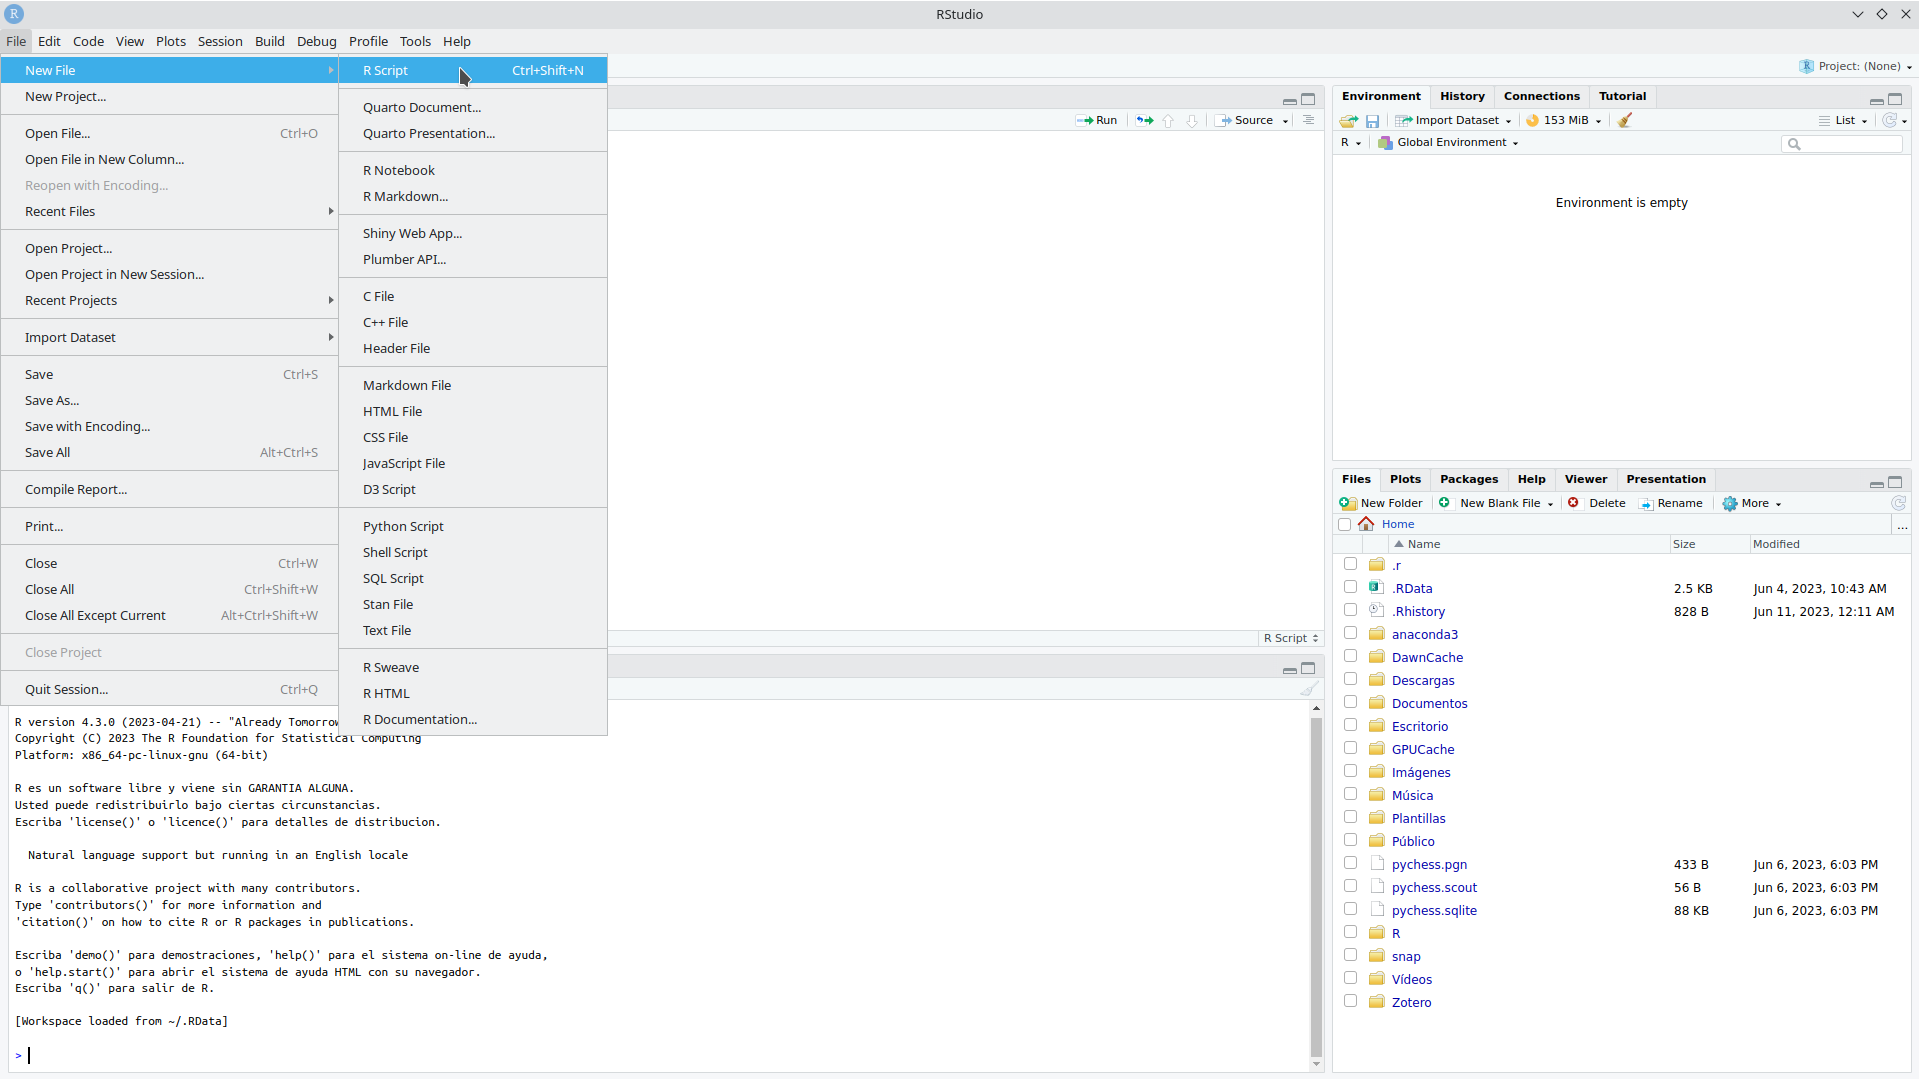
\includegraphics{images/Screenshot_20230611_001234.png}

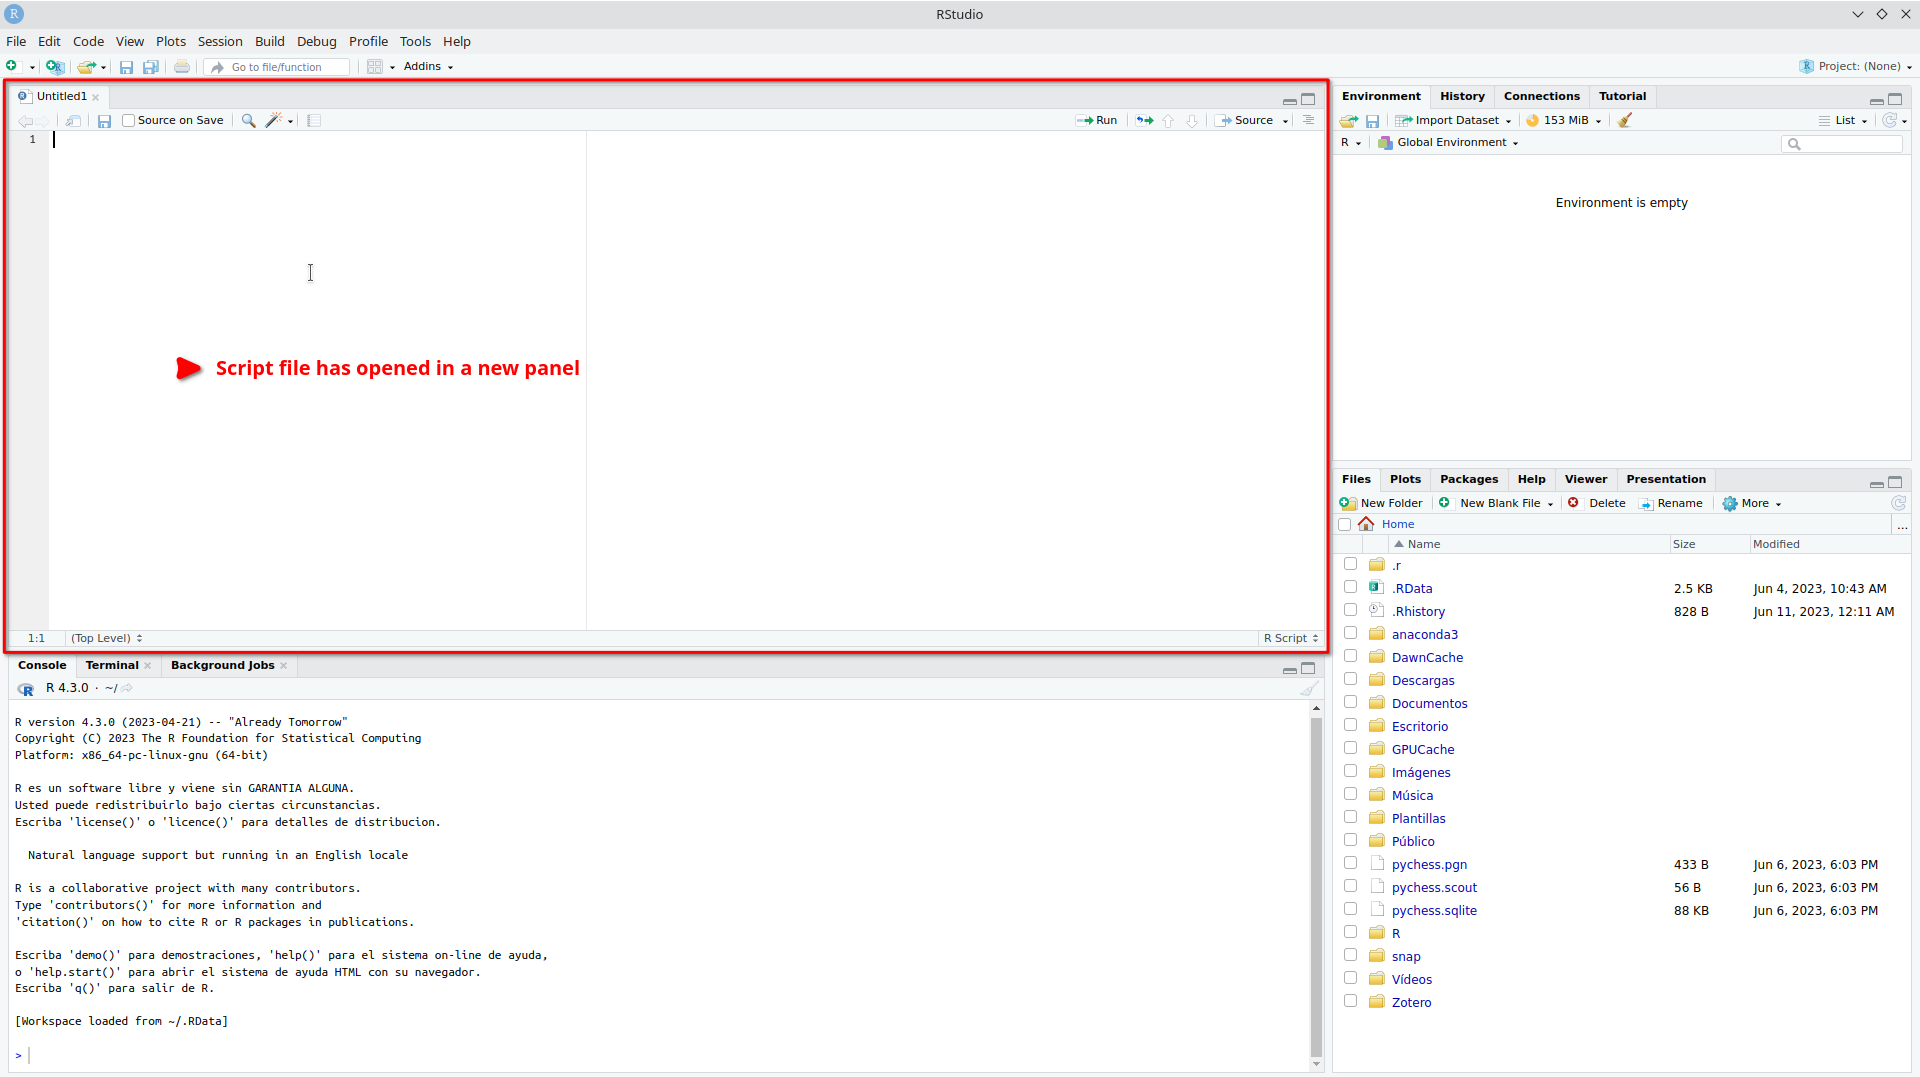
\includegraphics{images/Screenshot_20230611_001615.png}

\textbf{Paso 2: Escribir el código en el script}

Una vez que tenemos nuestro archivo de script abierto, podemos comenzar
a escribir nuestro código en R. Podemos utilizar cualquier comando o
función de R en el script para realizar análisis de datos, manipulación
de variables, visualización, entre otros. Es importante asegurarse de
que el código esté escrito correctamente y tenga una sintaxis válida.

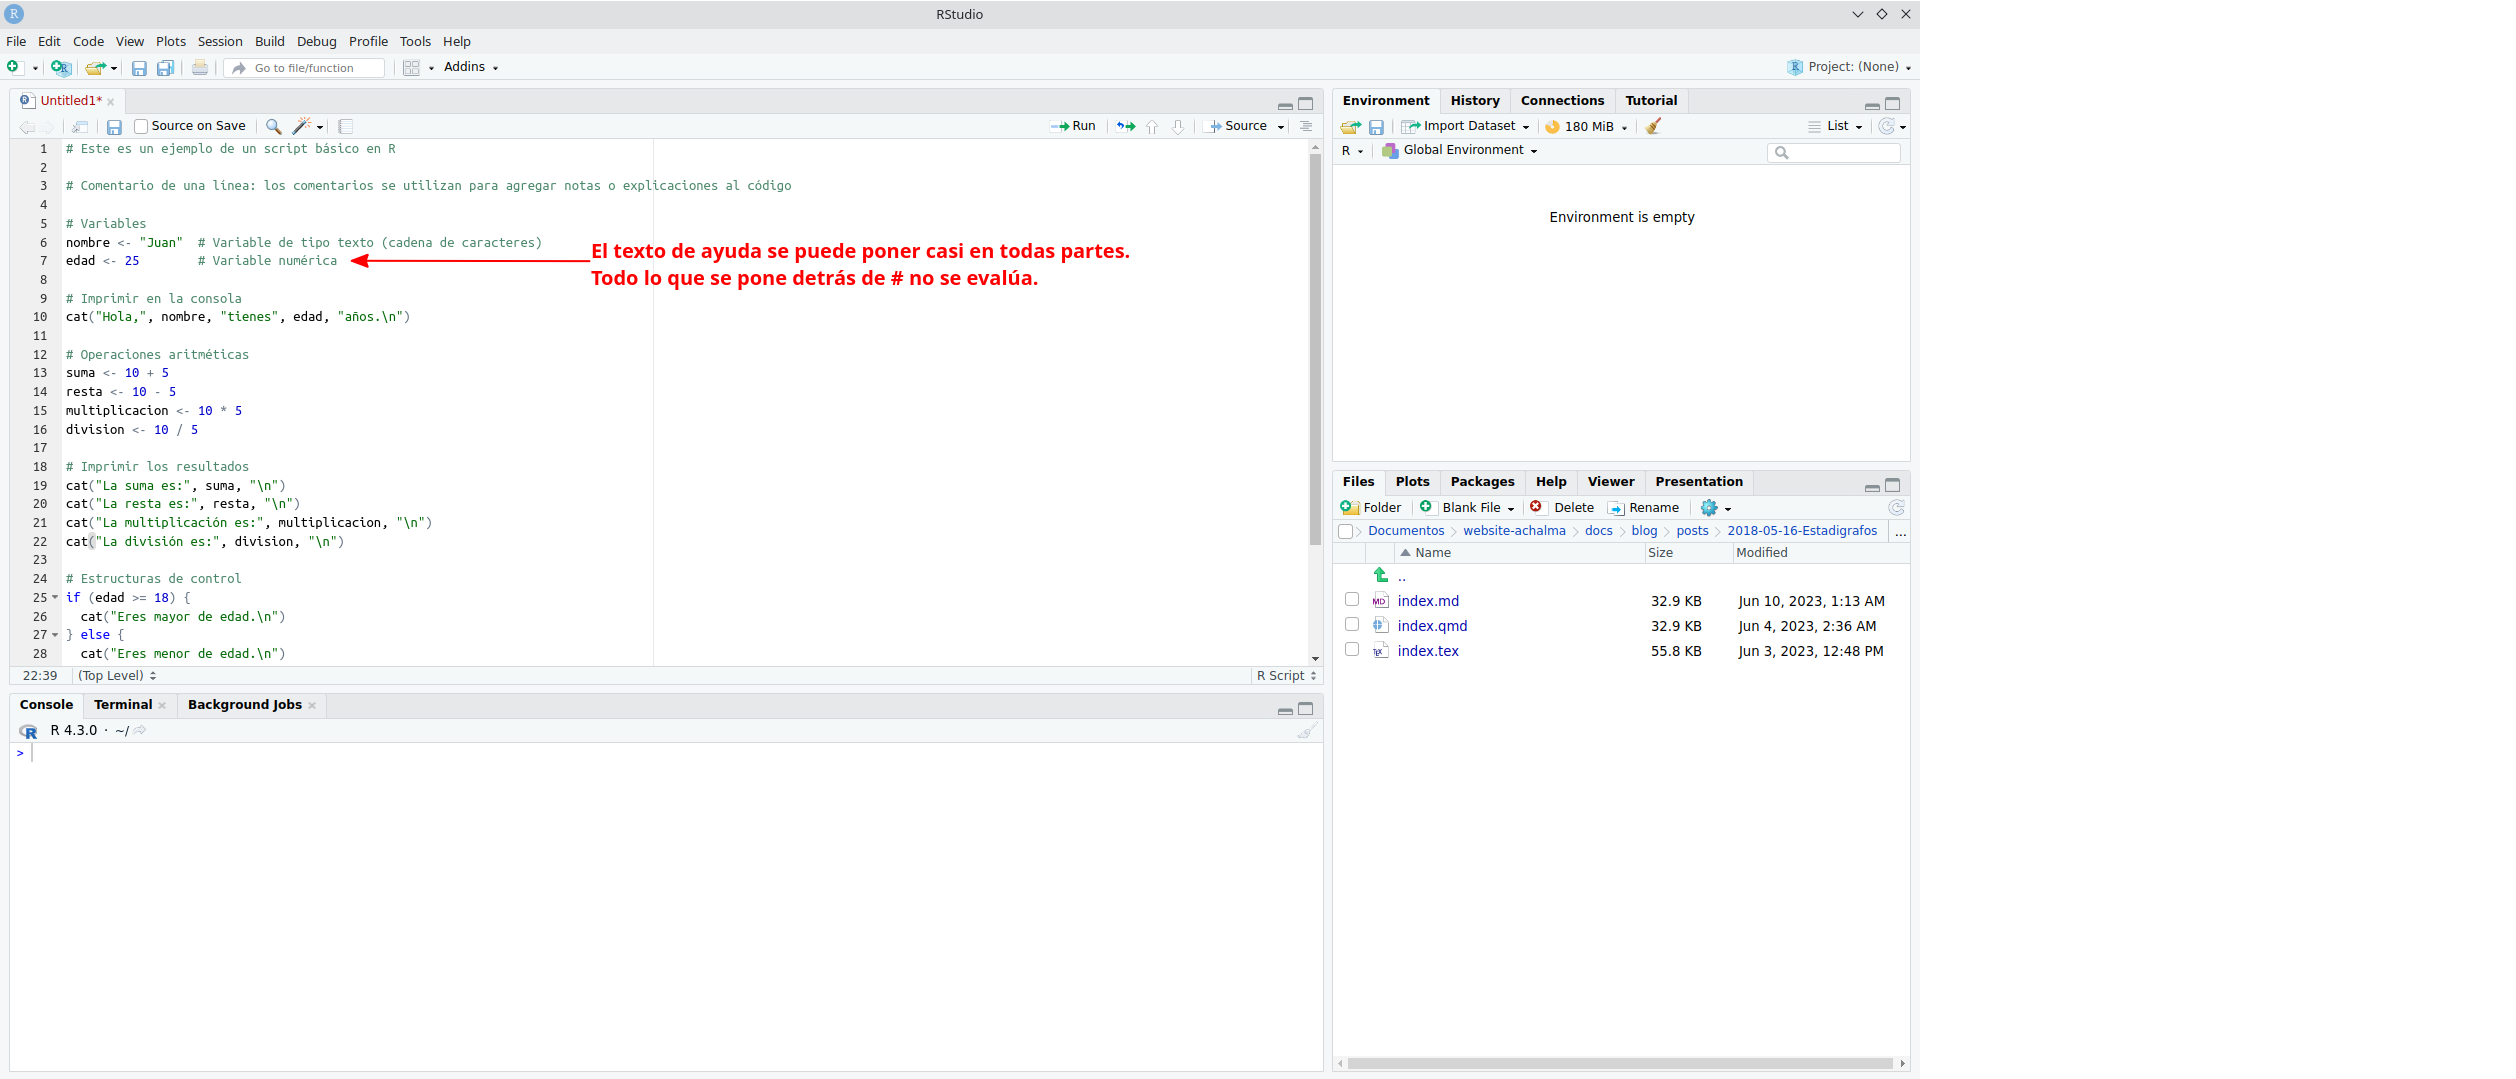
\includegraphics{images/Screenshot_20230611_004241.png}

\begin{Shaded}
\begin{Highlighting}[]
\CommentTok{\# Este es un ejemplo de un script básico en R}

\CommentTok{\# Comentario de una línea: los comentarios se utilizan para agregar notas o explicaciones al código}

\CommentTok{\# Variables}
\NormalTok{nombre }\OtherTok{\textless{}{-}} \StringTok{"Juan"} \CommentTok{\# Variable de tipo texto (cadena de caracteres)}
\NormalTok{edad }\OtherTok{\textless{}{-}} \DecValTok{25} \CommentTok{\# Variable numérica}

\CommentTok{\# Imprimir en la consola}
\FunctionTok{cat}\NormalTok{(}\StringTok{"Hola,"}\NormalTok{, nombre, }\StringTok{"tienes"}\NormalTok{, edad, }\StringTok{"años.}\SpecialCharTok{\textbackslash{}n}\StringTok{"}\NormalTok{)}

\CommentTok{\# Operaciones aritméticas}
\NormalTok{suma }\OtherTok{\textless{}{-}} \DecValTok{10} \SpecialCharTok{+} \DecValTok{5}
\NormalTok{resta }\OtherTok{\textless{}{-}} \DecValTok{10} \SpecialCharTok{{-}} \DecValTok{5}
\NormalTok{multiplicacion }\OtherTok{\textless{}{-}} \DecValTok{10} \SpecialCharTok{*} \DecValTok{5}
\NormalTok{division }\OtherTok{\textless{}{-}} \DecValTok{10} \SpecialCharTok{/} \DecValTok{5}

\CommentTok{\# Imprimir los resultados}
\FunctionTok{cat}\NormalTok{(}\StringTok{"La suma es:"}\NormalTok{, suma, }\StringTok{"}\SpecialCharTok{\textbackslash{}n}\StringTok{"}\NormalTok{)}
\FunctionTok{cat}\NormalTok{(}\StringTok{"La resta es:"}\NormalTok{, resta, }\StringTok{"}\SpecialCharTok{\textbackslash{}n}\StringTok{"}\NormalTok{)}
\FunctionTok{cat}\NormalTok{(}\StringTok{"La multiplicación es:"}\NormalTok{, multiplicacion, }\StringTok{"}\SpecialCharTok{\textbackslash{}n}\StringTok{"}\NormalTok{)}
\FunctionTok{cat}\NormalTok{(}\StringTok{"La división es:"}\NormalTok{, division, }\StringTok{"}\SpecialCharTok{\textbackslash{}n}\StringTok{"}\NormalTok{)}
\end{Highlighting}
\end{Shaded}

\textbf{Paso 3: Ejecutar el script}

Una vez que hemos escrito nuestro código en el archivo de script,
podemos ejecutarlo para obtener los resultados deseados. Para hacer
esto, podemos utilizar el atajo de teclado ``Ctrl + Enter'' o
simplemente hacer clic en el botón ``Ejecutar'' en la parte superior del
editor de texto.

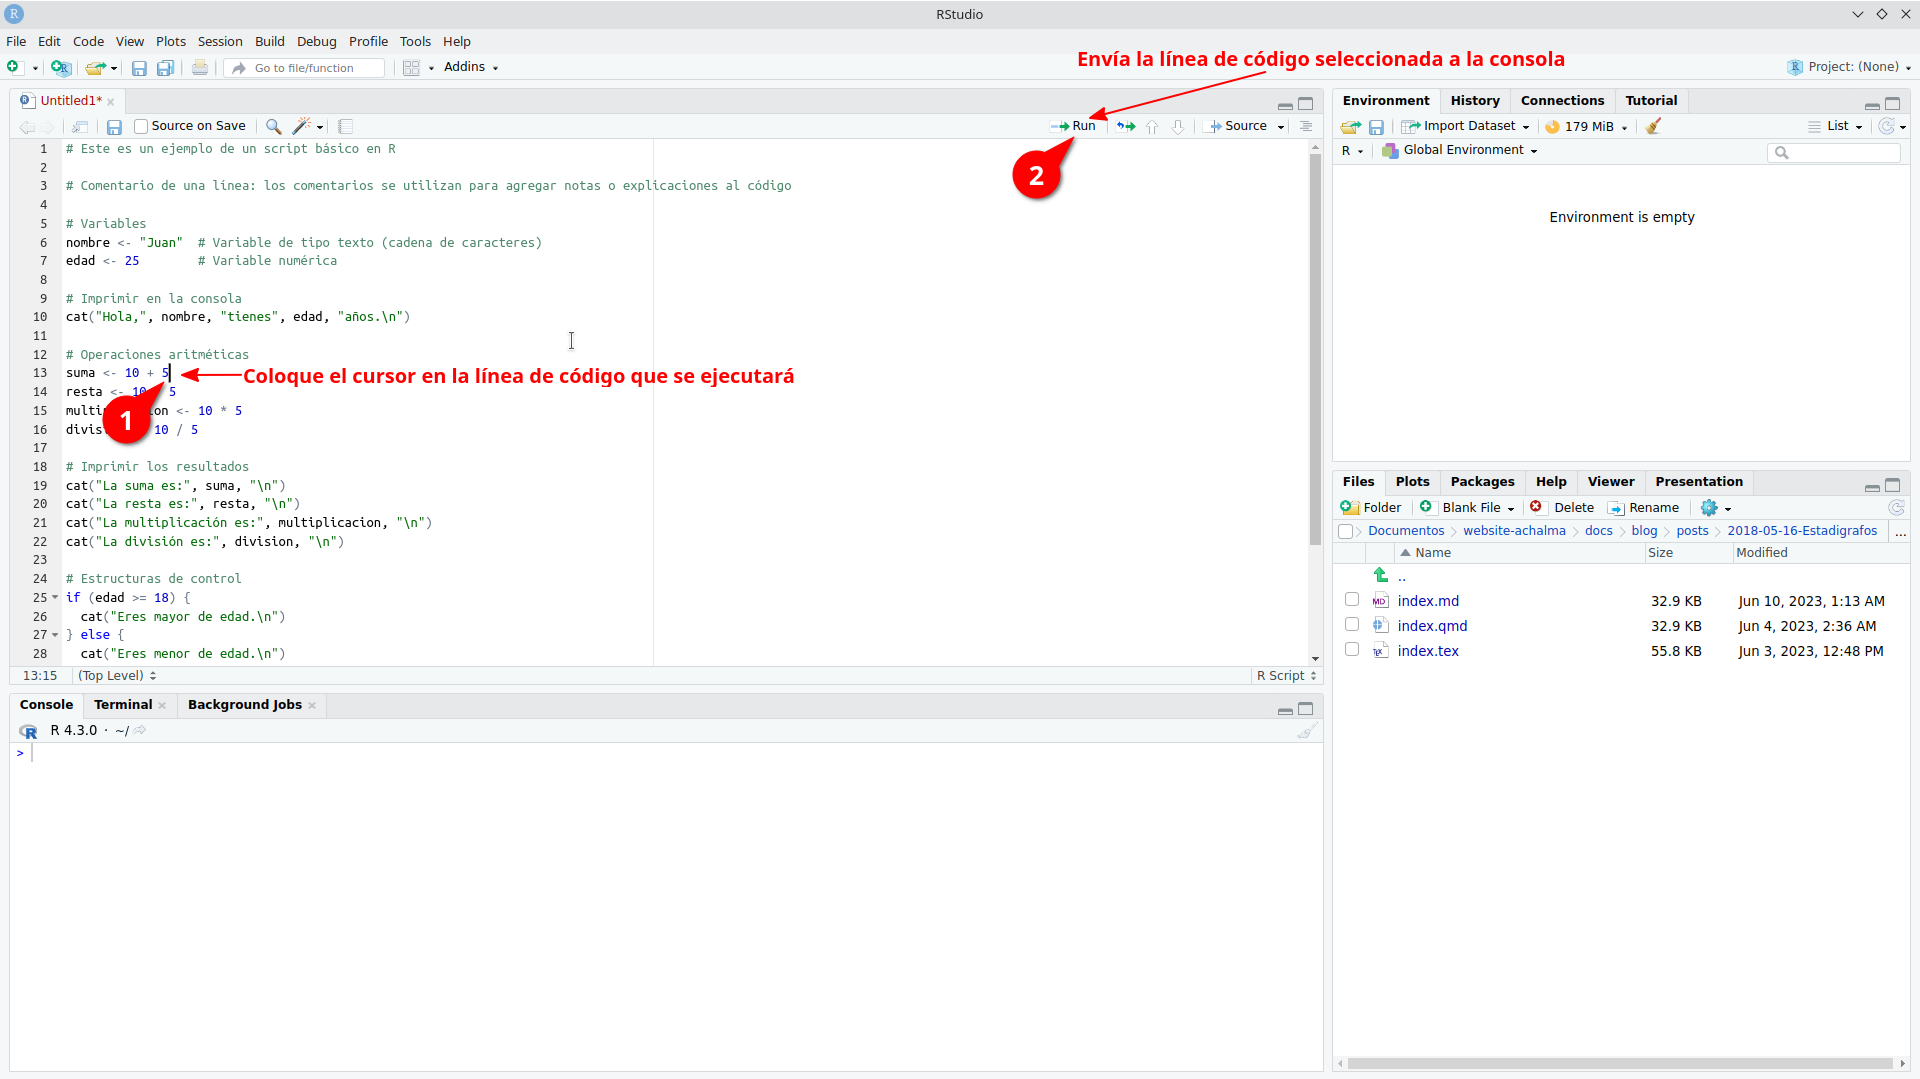
\includegraphics{images/Screenshot_20230611_005354.png}

RStudio ejecutará el código línea por línea y mostrará los resultados en
la consola.

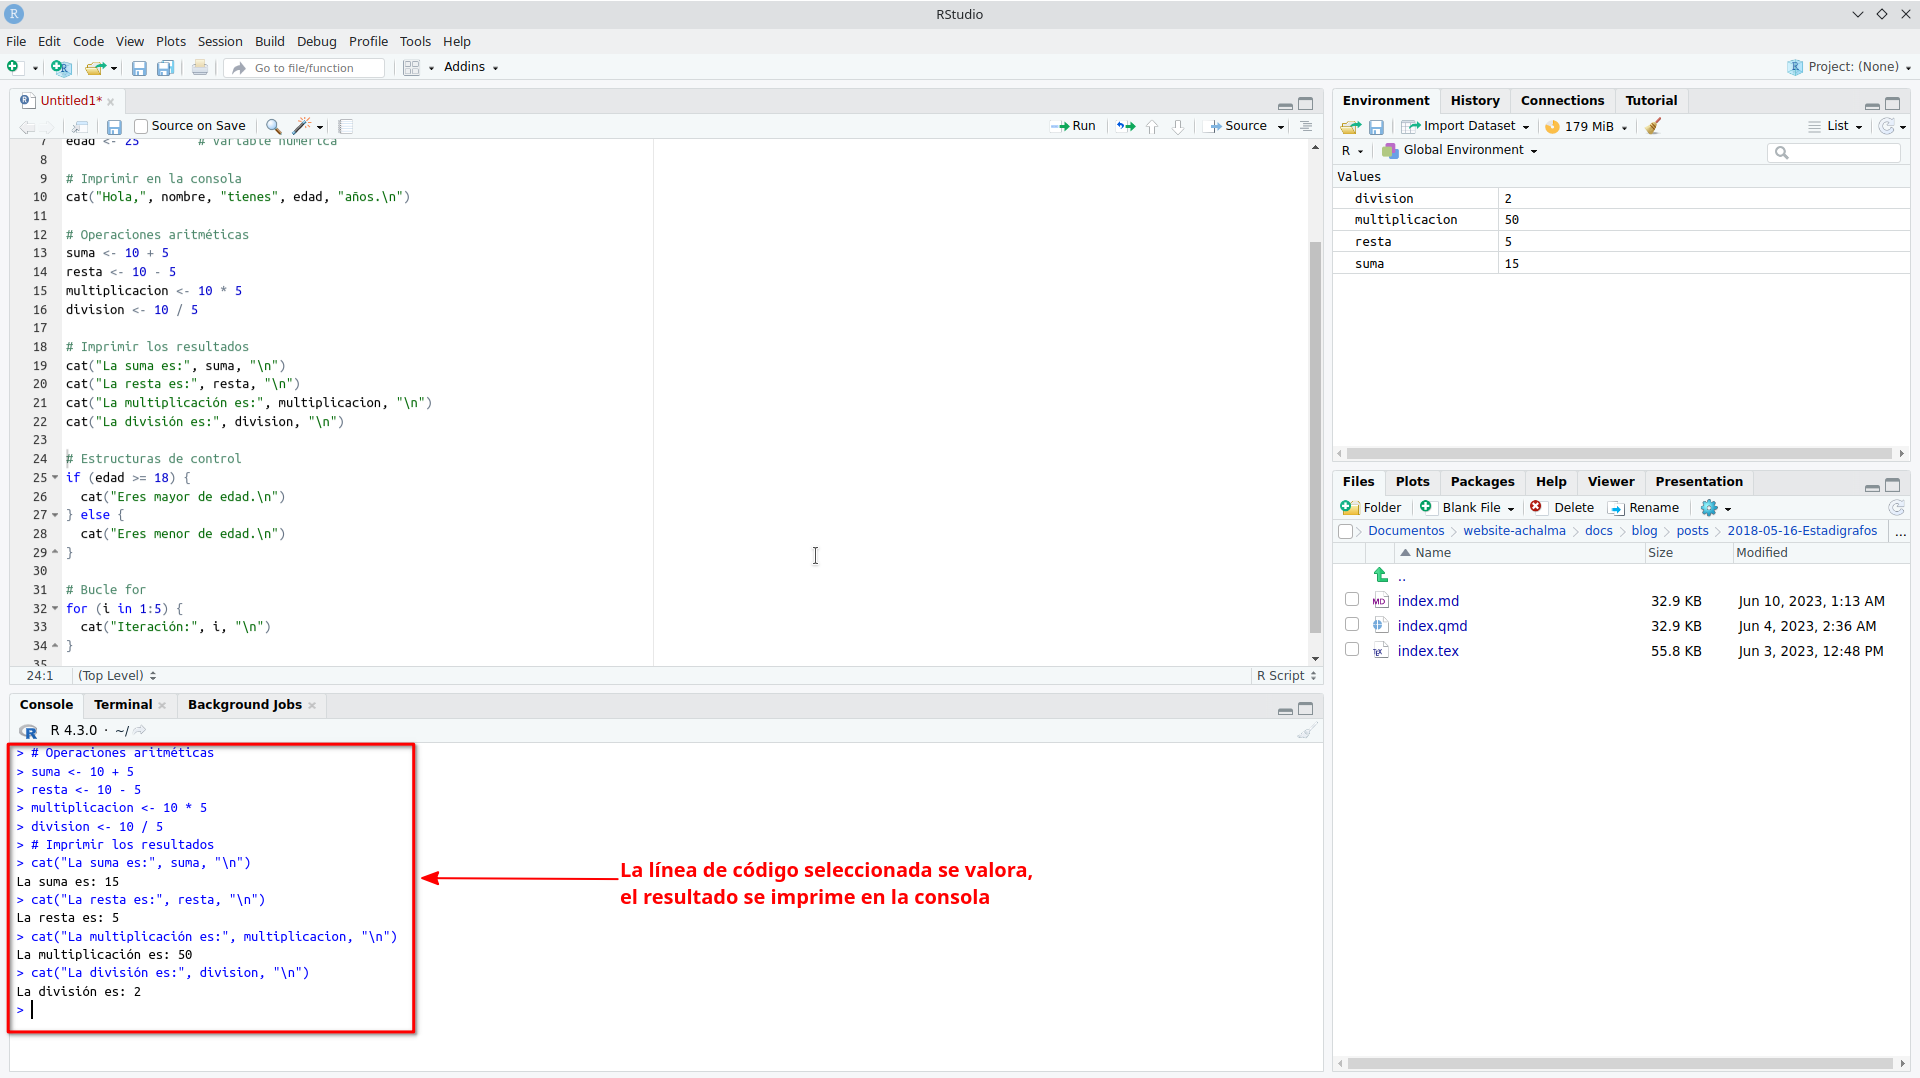
\includegraphics{images/Screenshot_20230611_010256.png}

\textbf{Paso 4: Guardar el script}

Es importante guardar regularmente nuestro script para evitar perder
nuestro trabajo. Para guardar el archivo de script, seleccionamos
``Archivo'' en la barra de menú y luego ``Guardar'' o ``Guardar como''.

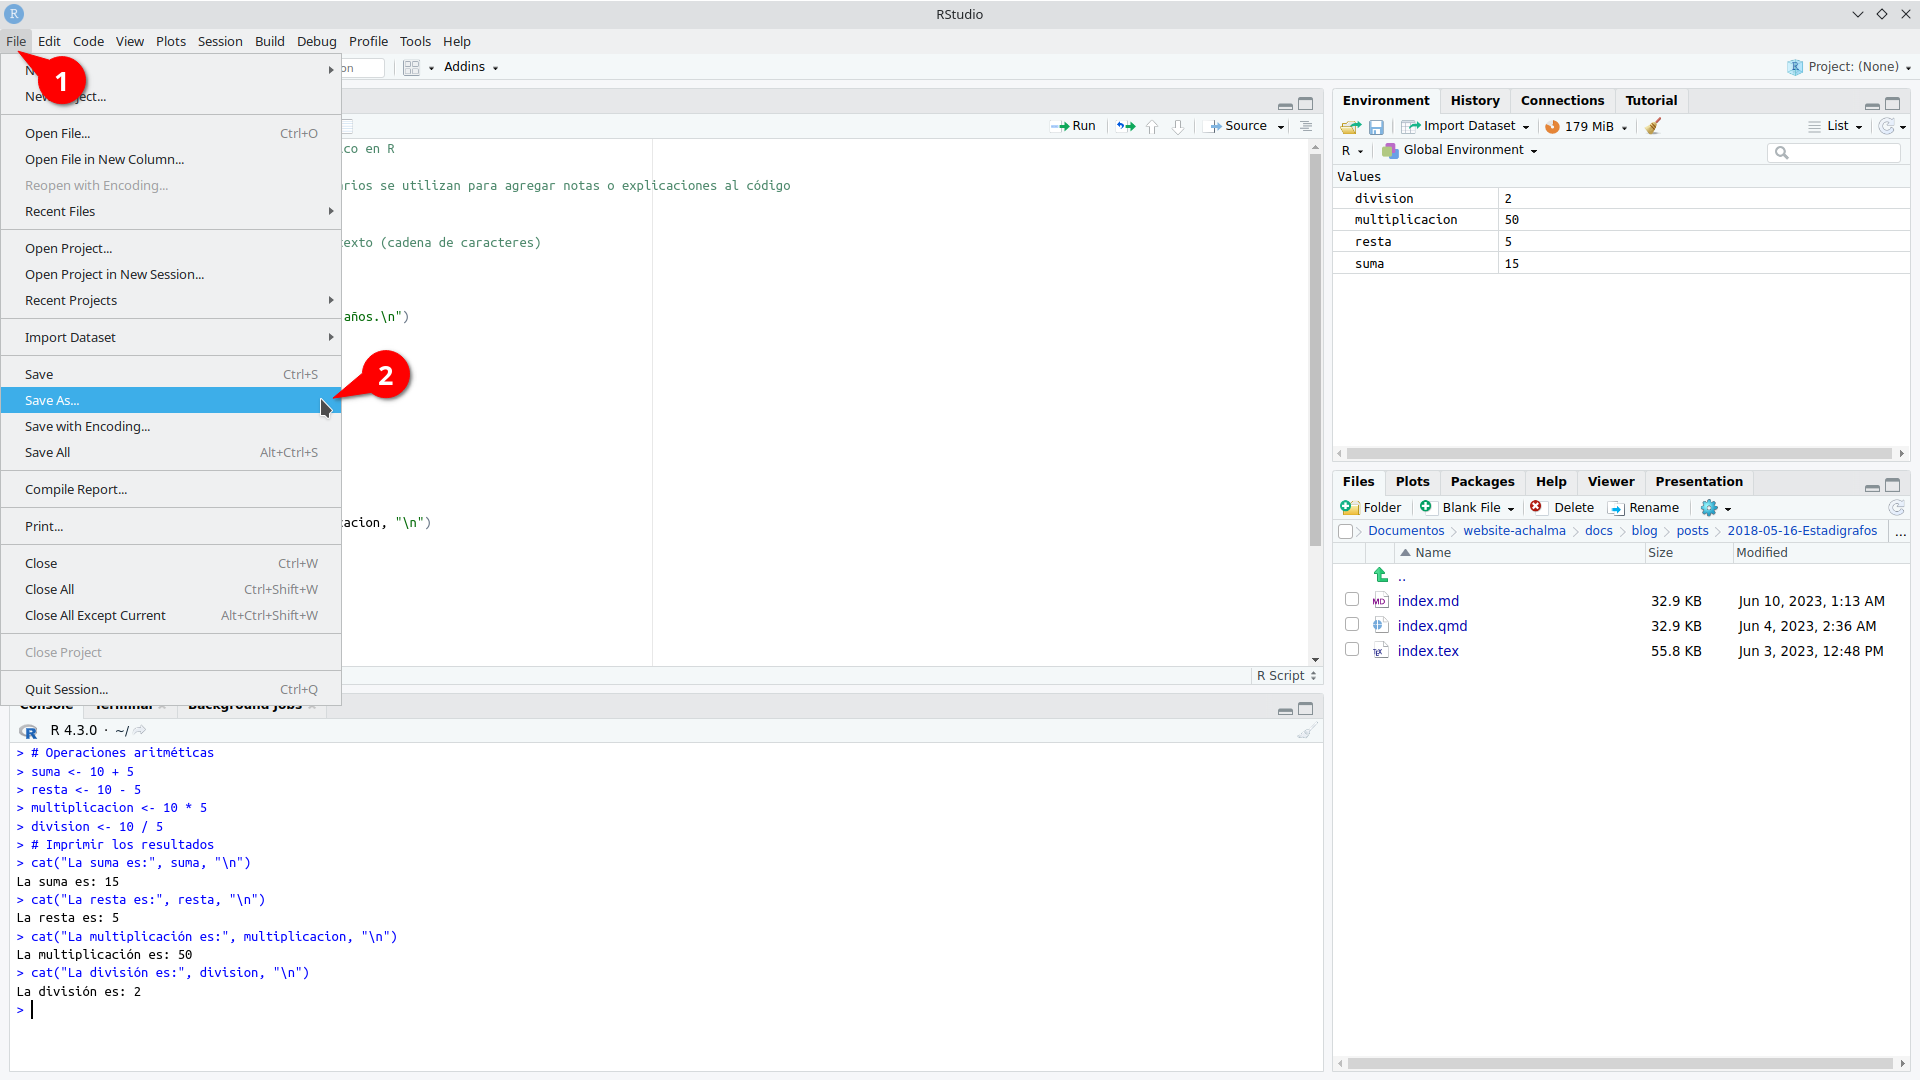
\includegraphics{images/Screenshot_20230611_010854.png}

Podemos elegir una ubicación y un nombre de archivo apropiados para
guardar nuestro script.

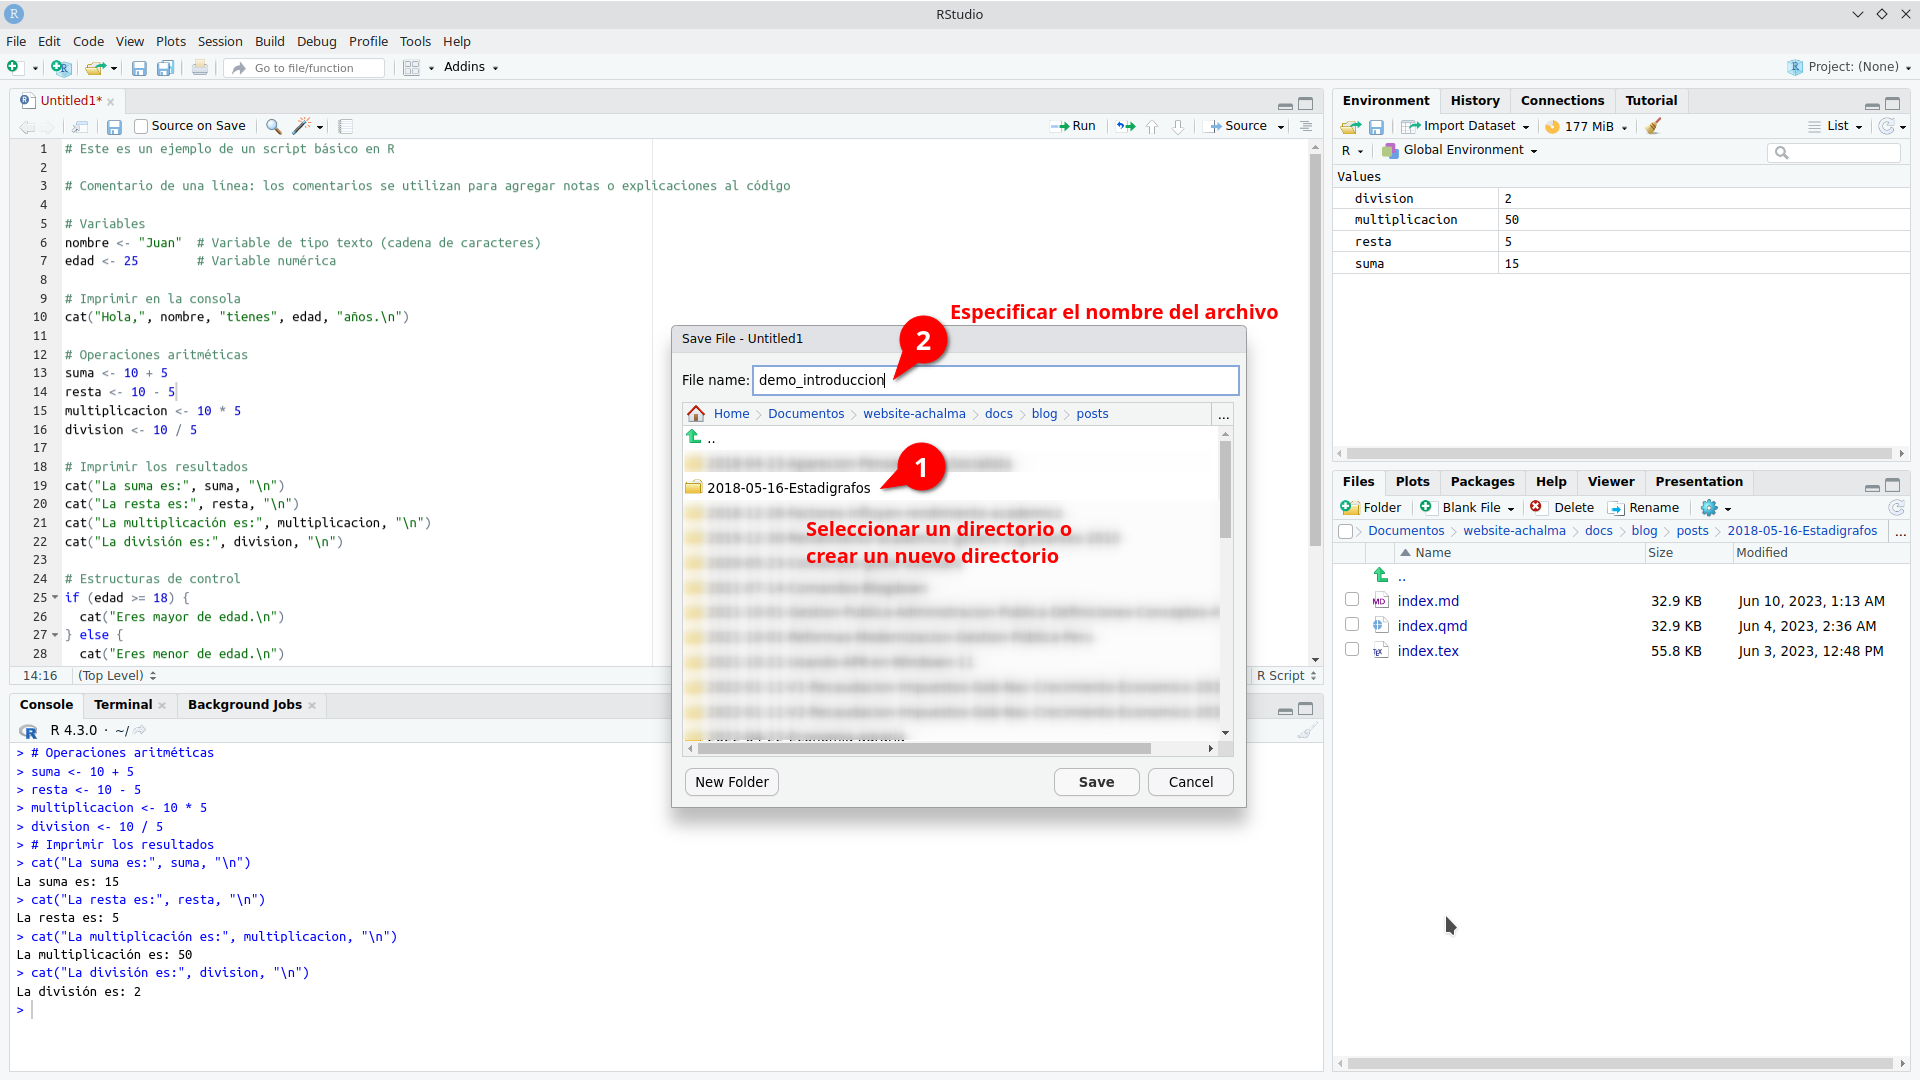
\includegraphics{images/Screenshot_20230611_012736.png}

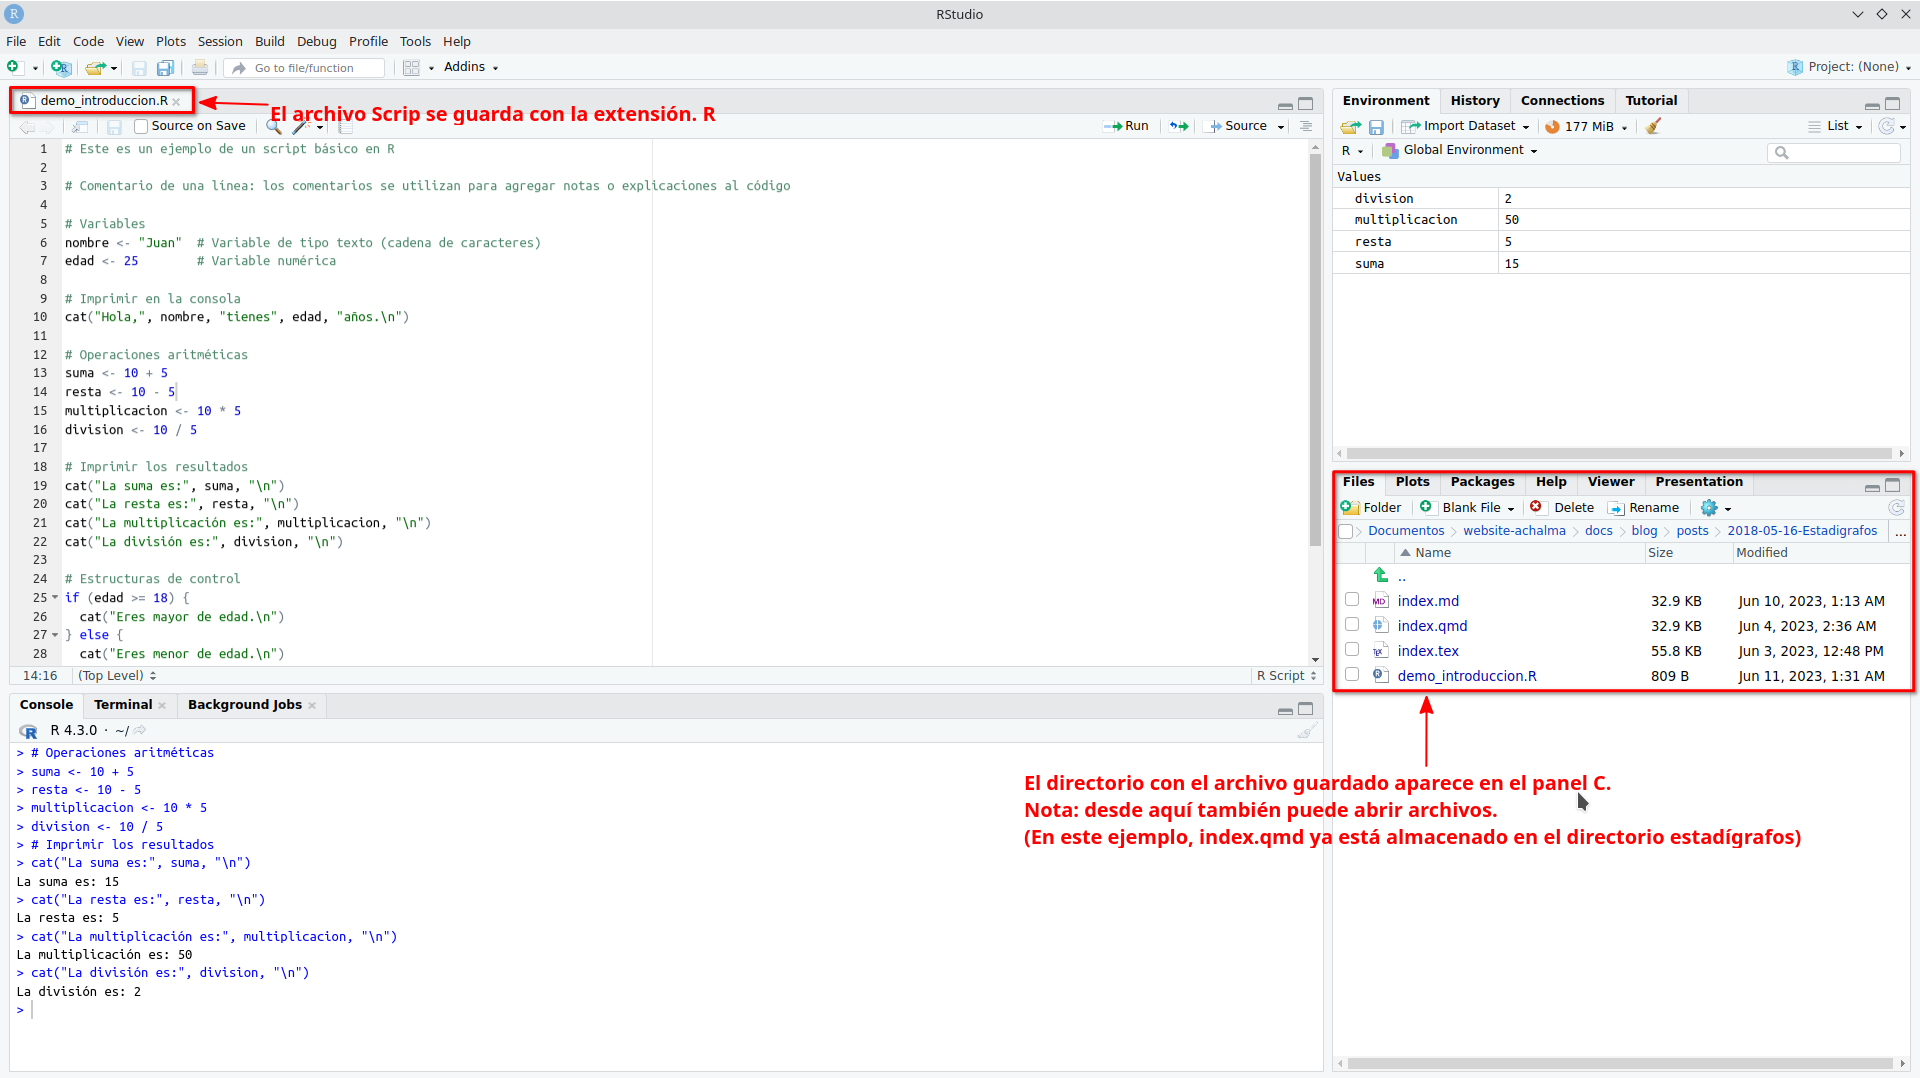
\includegraphics{images/Screenshot_20230611_013135.png}

\textbf{Paso 5: Continuar escribiendo y ejecutando el código}

Podemos continuar escribiendo y ejecutando más código en nuestro script
según nuestras necesidades. Podemos agregar nuevas líneas de código,
modificar las existentes o eliminar las que ya no necesitamos. Es
recomendable guardar el script regularmente a medida que realizamos
cambios.

\textbf{Paso 6: Exportar los resultados (opcional)}

Si deseamos guardar los resultados de nuestro análisis, podemos
exportarlos a archivos o formatos específicos. Por ejemplo, podemos
guardar tablas de datos en archivos CSV, gráficos en imágenes o informes
en formatos de texto. Esto nos permite compartir y utilizar los
resultados fuera de RStudio.

\begin{quote}
Recuerda que practicar y experimentar con diferentes comandos y
funciones en RStudio te ayudará a familiarizarte con el entorno y
mejorar tus habilidades de programación en R. ¡Diviértete explorando el
mundo del análisis de datos con RStudio!
\end{quote}

\hypertarget{shortcuts}{%
\subsection{Shortcuts}\label{shortcuts}}

Aquí tienes una tabla con algunos atajos de teclado útiles en RStudio
para usuarios de Ubuntu Linux:

\begin{longtable}[]{@{}
  >{\raggedright\arraybackslash}p{(\columnwidth - 2\tabcolsep) * \real{0.7222}}
  >{\raggedright\arraybackslash}p{(\columnwidth - 2\tabcolsep) * \real{0.2778}}@{}}
\toprule\noalign{}
\begin{minipage}[b]{\linewidth}\raggedright
Acción
\end{minipage} & \begin{minipage}[b]{\linewidth}\raggedright
Atajo de teclado
\end{minipage} \\
\midrule\noalign{}
\endhead
\bottomrule\noalign{}
\endlastfoot
Ejecutar el código / selección actual y saltar a la línea siguiente &
Ctrl + Enter \\
Ejecutar el código / selección actual y no saltar a la línea siguiente &
Alt + Enter \\
Ejecutar línea de código & Shift + Enter \\
Comentar/descomentar línea de código & Ctrl + Shift + C \\
Copiar línea de código & Ctrl + Shift + D \\
Pegar línea de código & Ctrl + Shift + V \\
Ir a la línea & Ctrl + G \\
Ir al inicio del documento & Ctrl + Home \\
Ir al final del documento & Ctrl + End \\
Completar código & Tab \\
Abrir ayuda & F1 \\
Guardar el archivo actual & Ctrl + S \\
Cerrar archivo & Ctrl + W \\
Deshacer & Ctrl + Z \\
Rehacer & Ctrl + Y \\
Abrir consola de R & Ctrl + Shift + Enter \\
Buscar en el archivo & Ctrl + F \\
Buscar y reemplazar en el archivo & Ctrl + Shift + F \\
Colapsar/expandir bloque de código & Ctrl + Shift + \\
Aumentar tamaño de fuente & Ctrl + + \\
Disminuir tamaño de fuente & Ctrl + - \\
Nuevo archivo Script R & Shift + Ctrl + N \\
Abrir archivo & Ctrl + O \\
Ejecutar todo el script & Ctrl + Alt + R \\
Ejecutar el código desde el principio hasta la línea actual & Ctrl + Alt
+ B \\
Ejecutar el código desde la línea actual hasta el final & Ctrl + Alt +
E \\
Mover el cursor al editor de código fuente & Ctrl + 1 \\
Mover el cursor a la consola & Ctrl + 2 \\
Eliminar selección actual & Ctrl + D \\
Limpiar consola & Ctrl + L \\
Navegar por el historial de la consola & arriba/abajo \\
Mover la línea de código arriba y abajo (evita el trabajo de copiar y
pegar) & Alt + arriba/abajo \\
Interrumpir el comando en ejecución & Esc \\
\end{longtable}

Estos atajos de teclado te ayudarán a agilizar tu flujo de trabajo en
RStudio en Ubuntu Linux. Recuerda que también puedes personalizar los
atajos de teclado según tus preferencias en la sección de configuración
de RStudio.

\hypertarget{espacio-de-trabajo-.rdata}{%
\subsection{Espacio de trabajo
(.Rdata)}\label{espacio-de-trabajo-.rdata}}

El espacio de trabajo en R consiste en todos los objetos que se crean o
cargan durante una sesión de R.

\hypertarget{creaciuxf3n-de-objetos-de-datos}{%
\subsubsection{Creación de objetos de
datos}\label{creaciuxf3n-de-objetos-de-datos}}

\begin{enumerate}
\def\labelenumi{\arabic{enumi}.}
\tightlist
\item
  Utiliza el operador de asignación (\texttt{\textless{}-}) para crear
  un objeto de datos. Por ejemplo:
  \texttt{mi\_objeto\ \textless{}-\ c(1,\ 2,\ 3,\ 4,\ 5)}.
\end{enumerate}

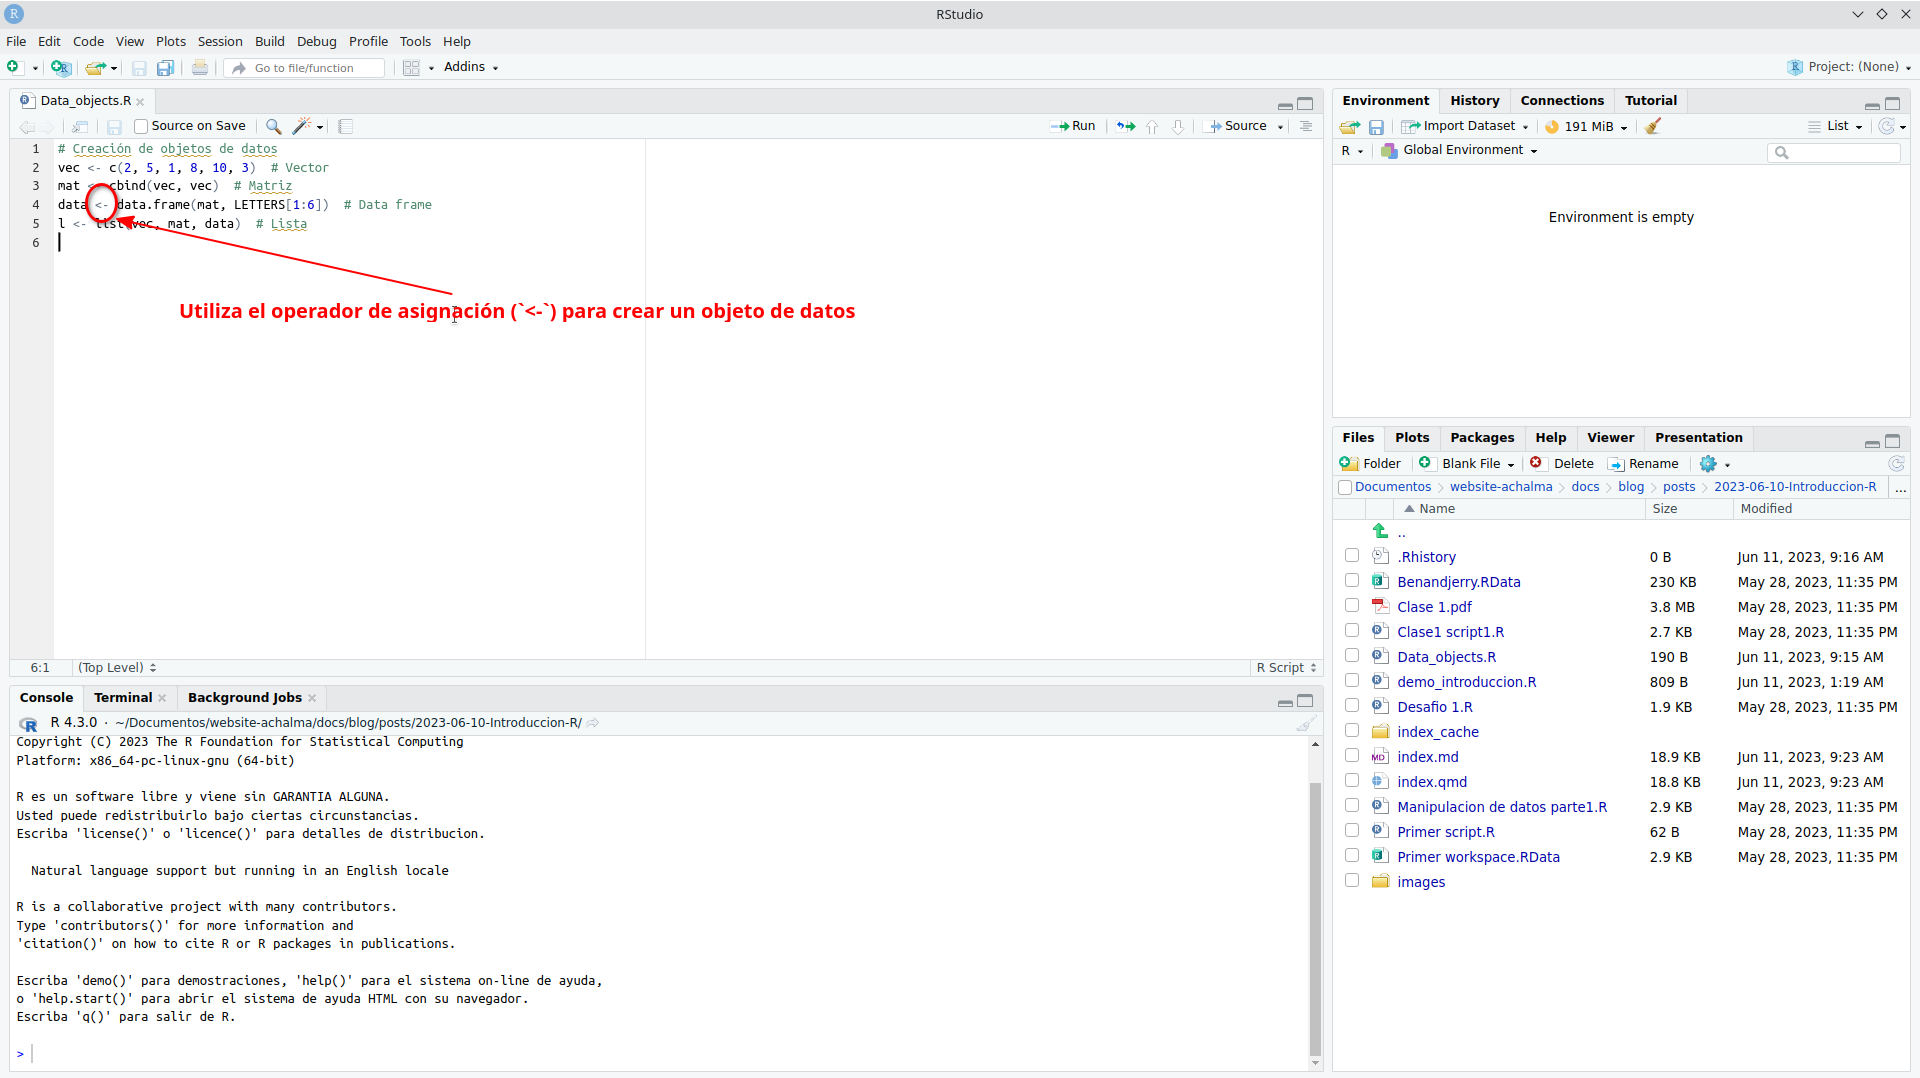
\includegraphics{images/Screenshot_20230611_092644.png}

\begin{enumerate}
\def\labelenumi{\arabic{enumi}.}
\setcounter{enumi}{1}
\tightlist
\item
  Selecciona todo el código que contiene los objetos de datos y
  ejecútalo en la consola de RStudio.
\end{enumerate}

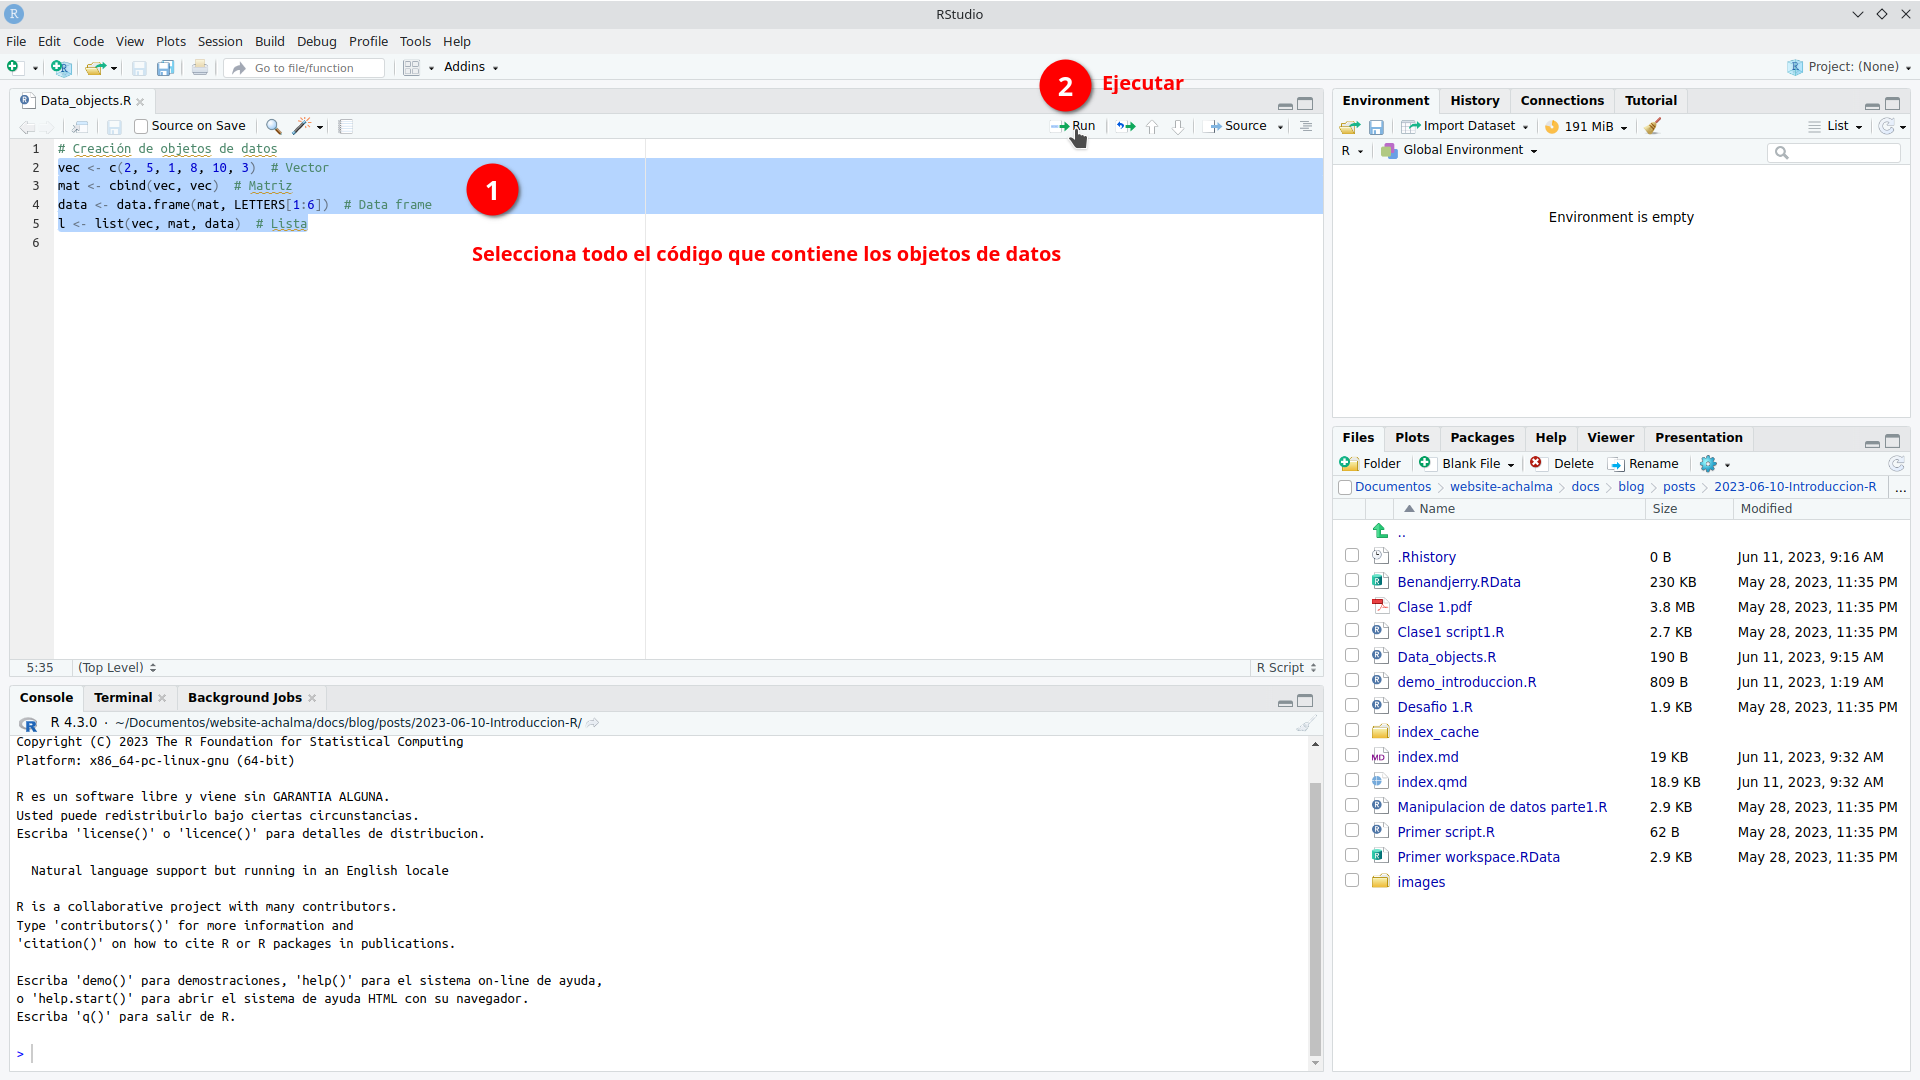
\includegraphics{images/Screenshot_20230611_093536.png}

\begin{enumerate}
\def\labelenumi{\arabic{enumi}.}
\setcounter{enumi}{2}
\tightlist
\item
  El código se evaluará y los objetos de datos se crearán en el espacio
  de trabajo. Sin embargo, no verás ningún resultado en la consola.
\end{enumerate}

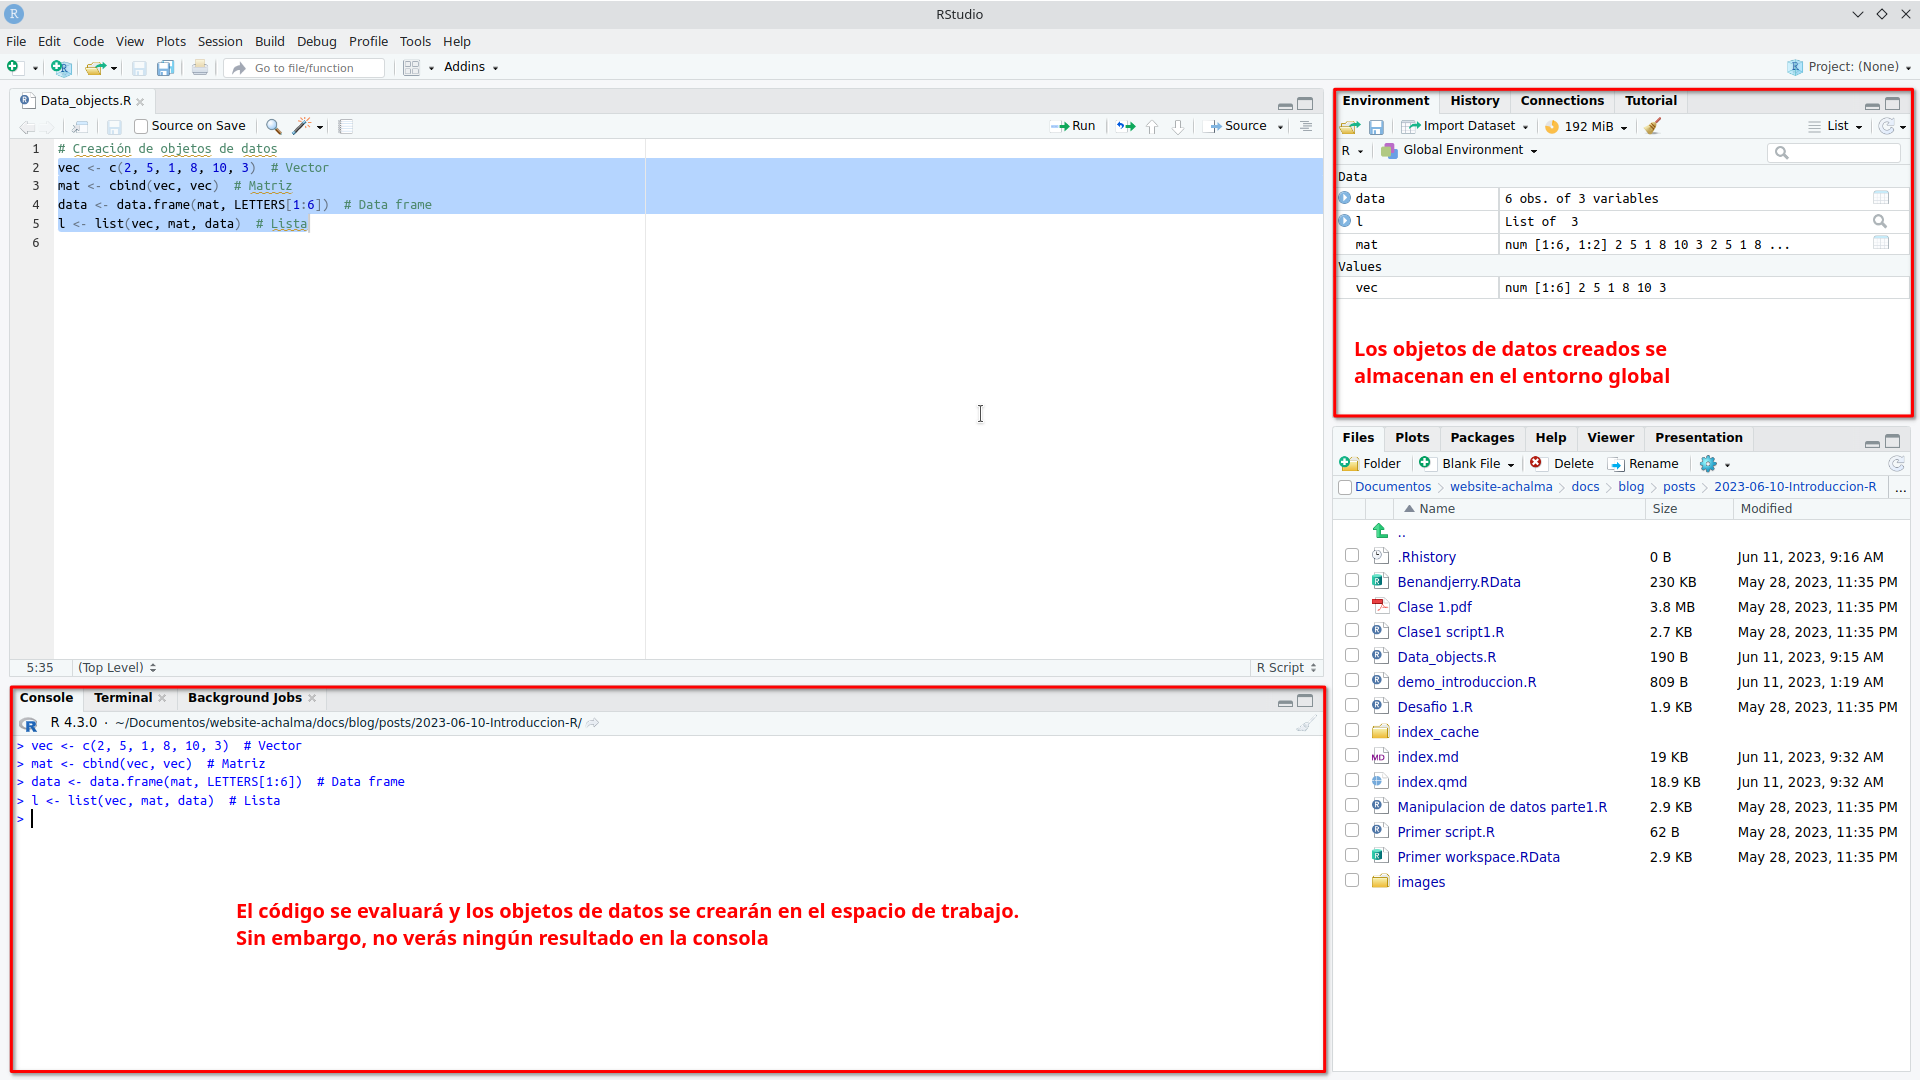
\includegraphics{images/Screenshot_20230611_094001.png}

Los objetos de datos creados se almacenan en el entorno global, que es
parte del espacio de trabajo de R.

\hypertarget{inspecciuxf3n-de-objetos-de-datos}{%
\subsubsection{Inspección de objetos de
datos}\label{inspecciuxf3n-de-objetos-de-datos}}

Puedes inspeccionar los objetos de datos haciendo clic sobre ellos en el
panel de entorno o en el panel de objetos. Esto abrirá una vista previa
del objeto en un nuevo archivo. Ten en cuenta que esta vista previa no
afecta los objetos en el espacio de trabajo y se puede cerrar sin perder
ninguna información.

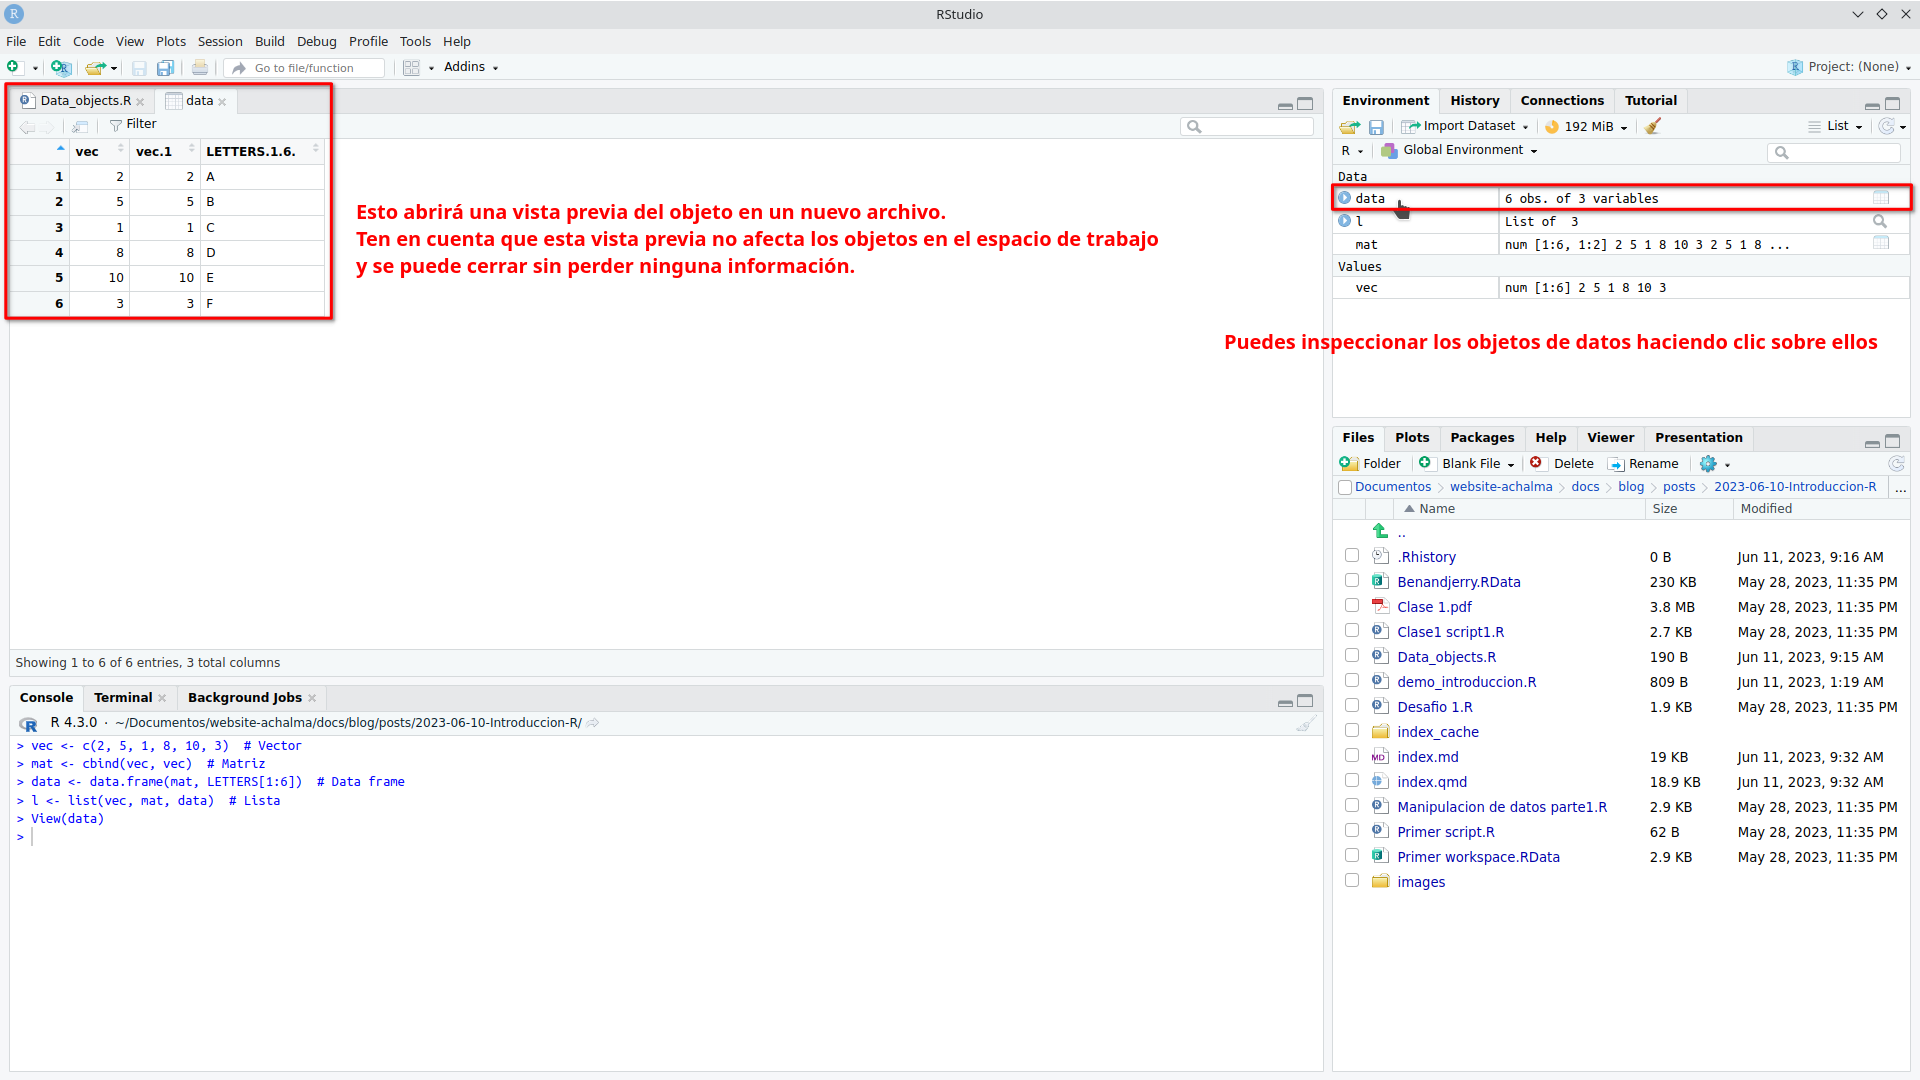
\includegraphics{images/Screenshot_20230611_094530.png}

\hypertarget{guardado-del-espacio-de-trabajo}{%
\subsubsection{Guardado del espacio de
trabajo}\label{guardado-del-espacio-de-trabajo}}

En RStudio, puedes guardar todos los objetos en tu espacio de trabajo en
un archivo llamado \texttt{.Rdata}. Esta función te permite almacenar y
cargar el espacio de trabajo completo en futuras sesiones de RStudio.

Para guardar el espacio de trabajo, simplemente ve al menú ``Session'' y
selecciona ``Save Workspace As\ldots{}''. A continuación, elige la
ubicación y el nombre de archivo deseados para guardar el archivo
\texttt{.Rdata}.

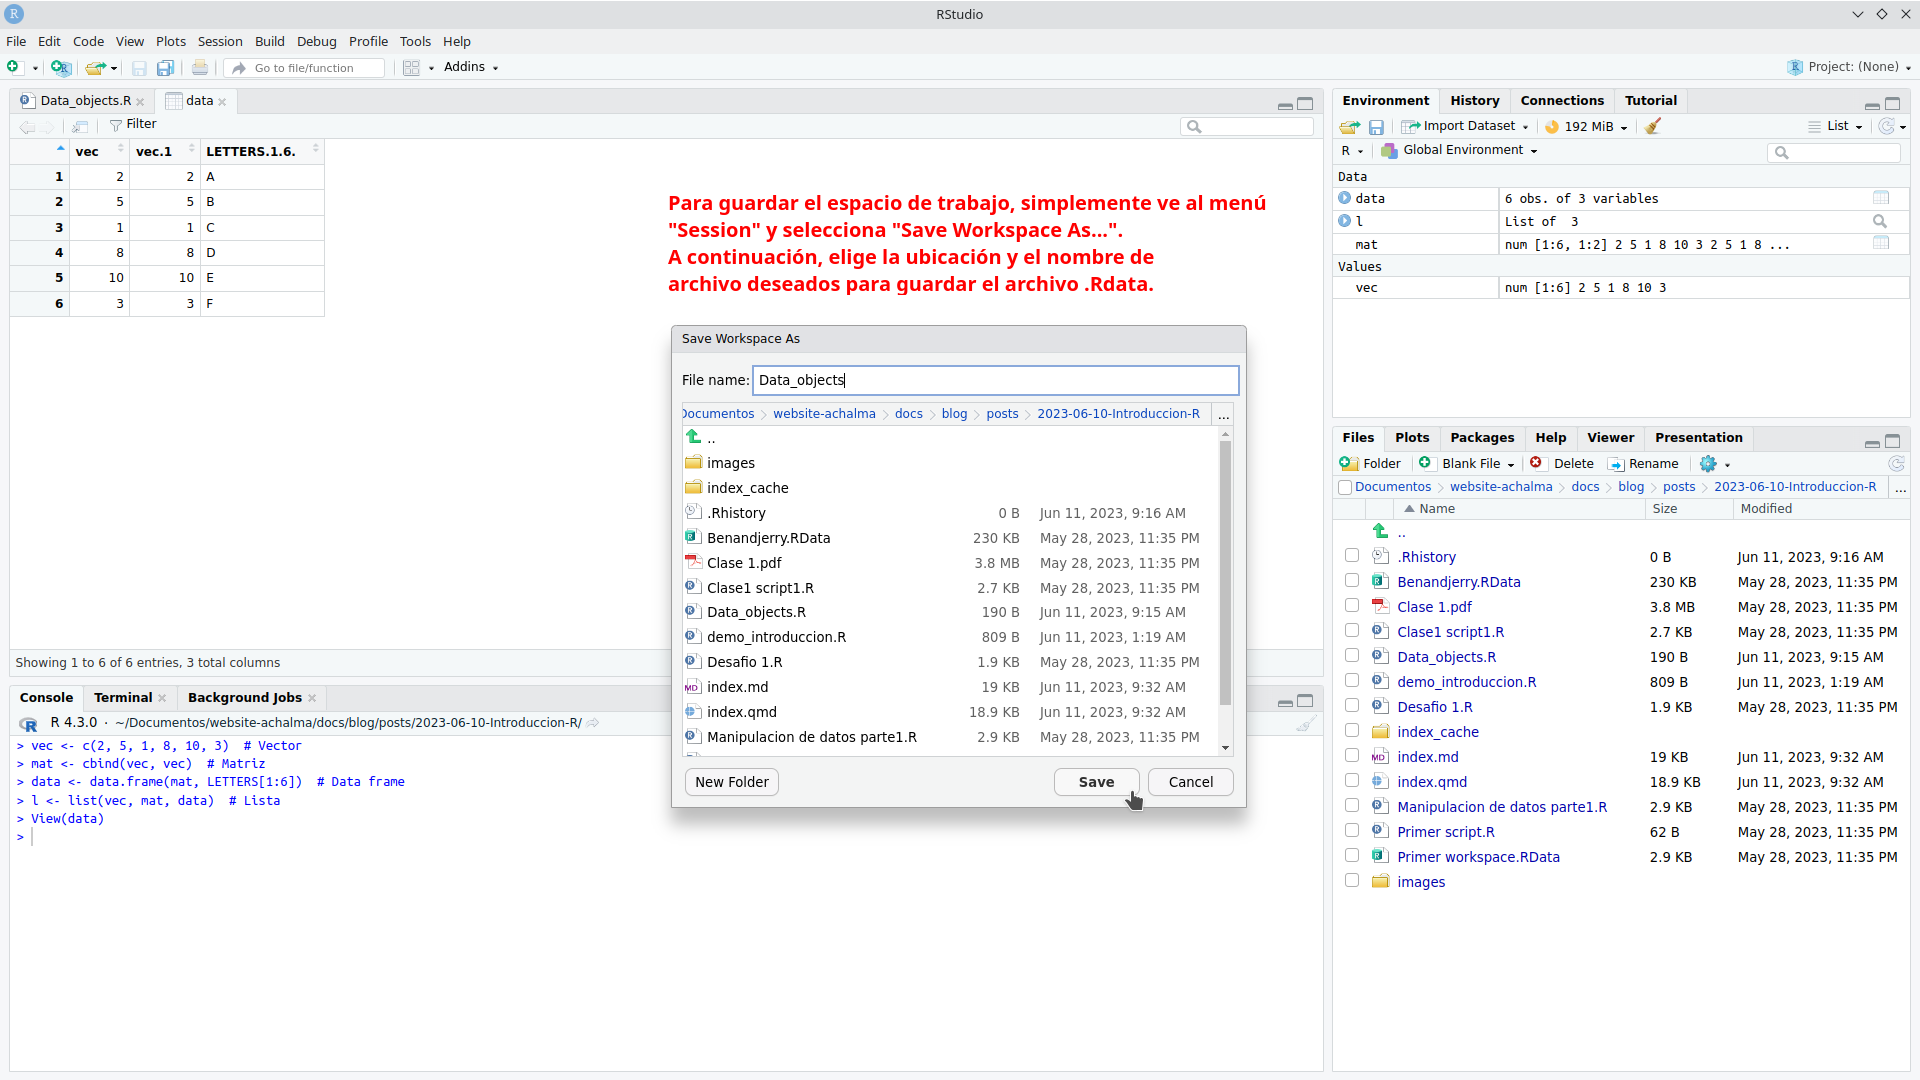
\includegraphics{images/Screenshot_20230611_095350.png}

Esta función es especialmente útil cuando trabajas en proyectos largos o
cuando deseas retomar tu trabajo en otro momento sin tener que volver a
crear o cargar manualmente todos los objetos y configuraciones.

\begin{quote}
Recuerda que al guardar y cargar el espacio de trabajo, asegúrate de
mantener un respaldo de tus archivos en caso de cualquier eventualidad.
¡Disfruta de la conveniencia de mantener tus objetos y configuraciones
en tu espacio de trabajo guardado!
\end{quote}

\hypertarget{carga-del-espacio-de-trabajo}{%
\subsubsection{Carga del espacio de
trabajo}\label{carga-del-espacio-de-trabajo}}

Para cargar el espacio de trabajo previamente guardado, sigue estos
pasos:

\begin{enumerate}
\def\labelenumi{\arabic{enumi}.}
\tightlist
\item
  Abre RStudio y ve al menú ``Session'' en la barra de herramientas
  superior.
\item
  Selecciona la opción ``Cargar'' del menú desplegable.
\item
  Aparecerá una ventana emergente que te permite buscar el archivo
  \texttt{.Rdata} que contiene tu espacio de trabajo guardado. Navega
  hasta la ubicación donde guardaste el archivo.
\item
  Selecciona el archivo \texttt{.Rdata} y haz clic en el botón
  ``Abrir''.
\item
  RStudio cargará automáticamente el archivo y restaurará todos los
  objetos y sus valores en tu entorno de trabajo actual.
\end{enumerate}

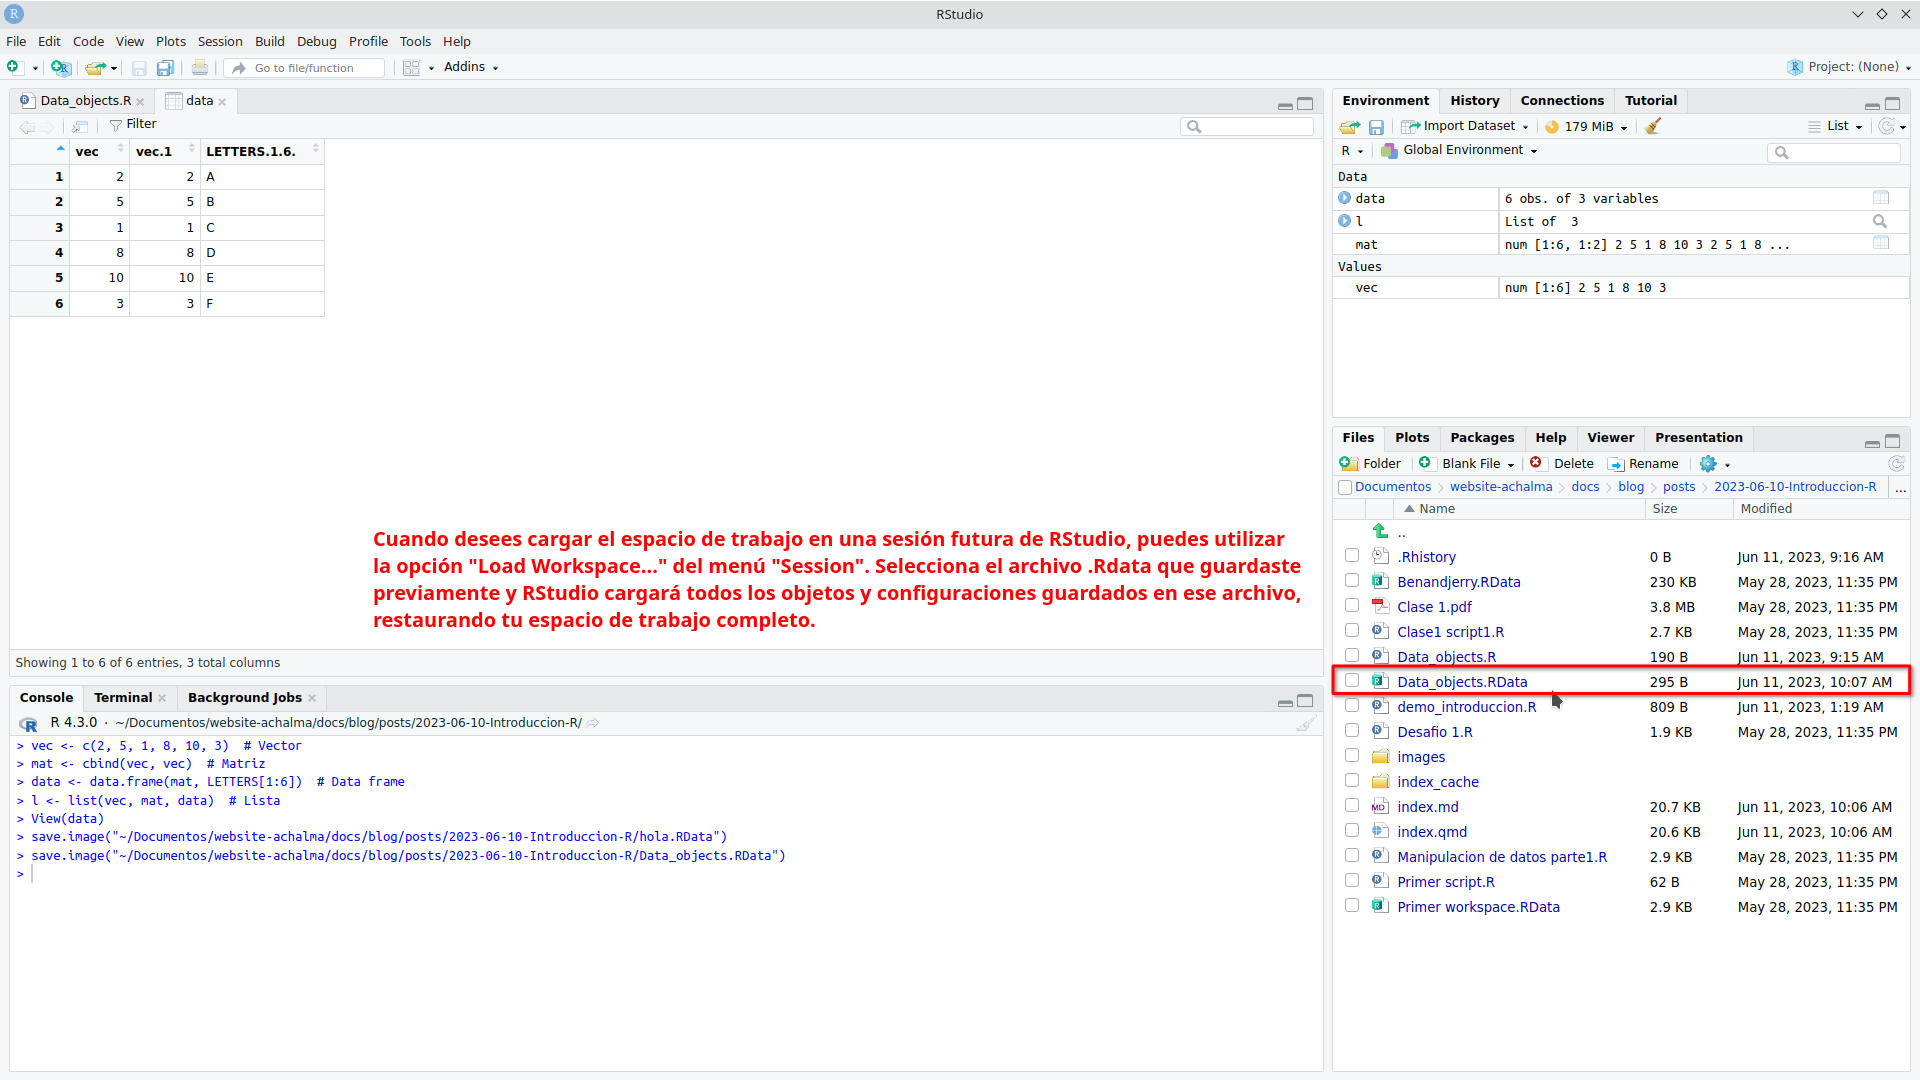
\includegraphics{images/Screenshot_20230611_100949.png}

Una vez completados estos pasos, podrás acceder a todos los objetos y
continuar trabajando con ellos como lo hiciste en la sesión en la que
guardaste el espacio de trabajo.

\begin{quote}
¡Con esta opción de carga, podrás retomar fácilmente tus proyectos
anteriores y continuar donde lo dejaste sin tener que volver a crear los
objetos desde cero!
\end{quote}

\hypertarget{historial-.rhistory}{%
\subsection{Historial (.Rhistory)}\label{historial-.rhistory}}

El archivo de historial es un archivo de texto que registra todos los
comandos ejecutados durante una sesión de RStudio.

\hypertarget{inspecciuxf3n-del-historial-de-comandos}{%
\subsubsection{Inspección del historial de
comandos}\label{inspecciuxf3n-del-historial-de-comandos}}

Puedes ver el historial de comandos ejecutados durante tu sesión de
trabajo haciendo clic en la pestaña ``History'' en la parte superior
derecha de la ventana de RStudio. Aquí encontrarás una lista de todos
los comandos ejecutados, lo que te permite revisarlos y volver a
utilizarlos según sea necesario.

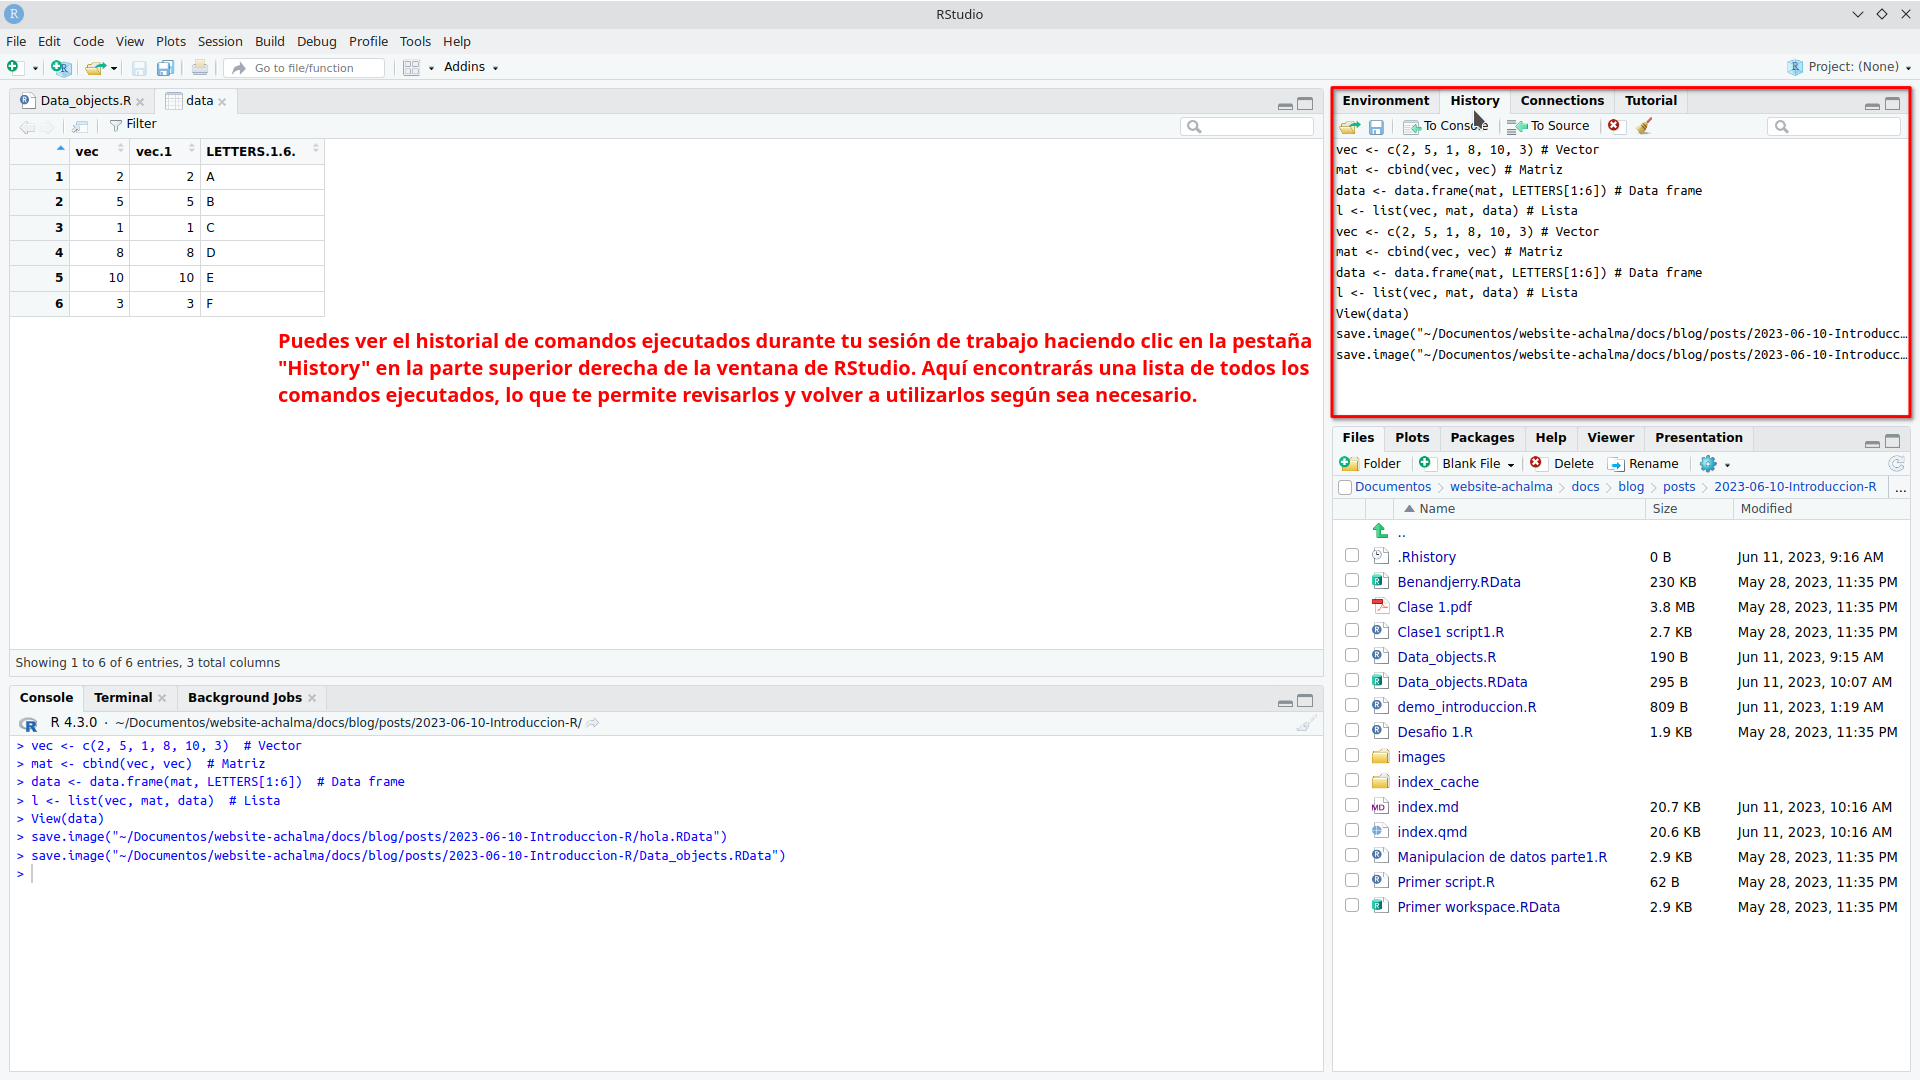
\includegraphics{images/Screenshot_20230611_101644.png}

\hypertarget{guardado-del-historial-de-comandos}{%
\subsubsection{Guardado del historial de
comandos}\label{guardado-del-historial-de-comandos}}

Si deseas guardar tu historial de comandos, puedes hacerlo en cualquier
momento durante tu sesión de trabajo. Esto te permitirá acceder a tus
comandos previos en futuras sesiones.

Si deseas guardar tu historial de comandos en RStudio, sigue estos
pasos:

\begin{enumerate}
\def\labelenumi{\arabic{enumi}.}
\tightlist
\item
  En el panel de superior derecha selecciona la opción ``Save History''
  (Guardar Historial).
\item
  Aparecerá una ventana emergente que te permitirá seleccionar la
  ubicación y el nombre de archivo para guardar tu historial de
  comandos. El archivo tendrá una extensión \texttt{.Rhistory} por
  defecto.
\item
  Elige la ubicación donde deseas guardar el archivo y asigna un nombre
  descriptivo para identificarlo fácilmente.
\item
  Haz clic en el botón ``Guardar'' para guardar el historial de comandos
  en el archivo seleccionado.
\end{enumerate}

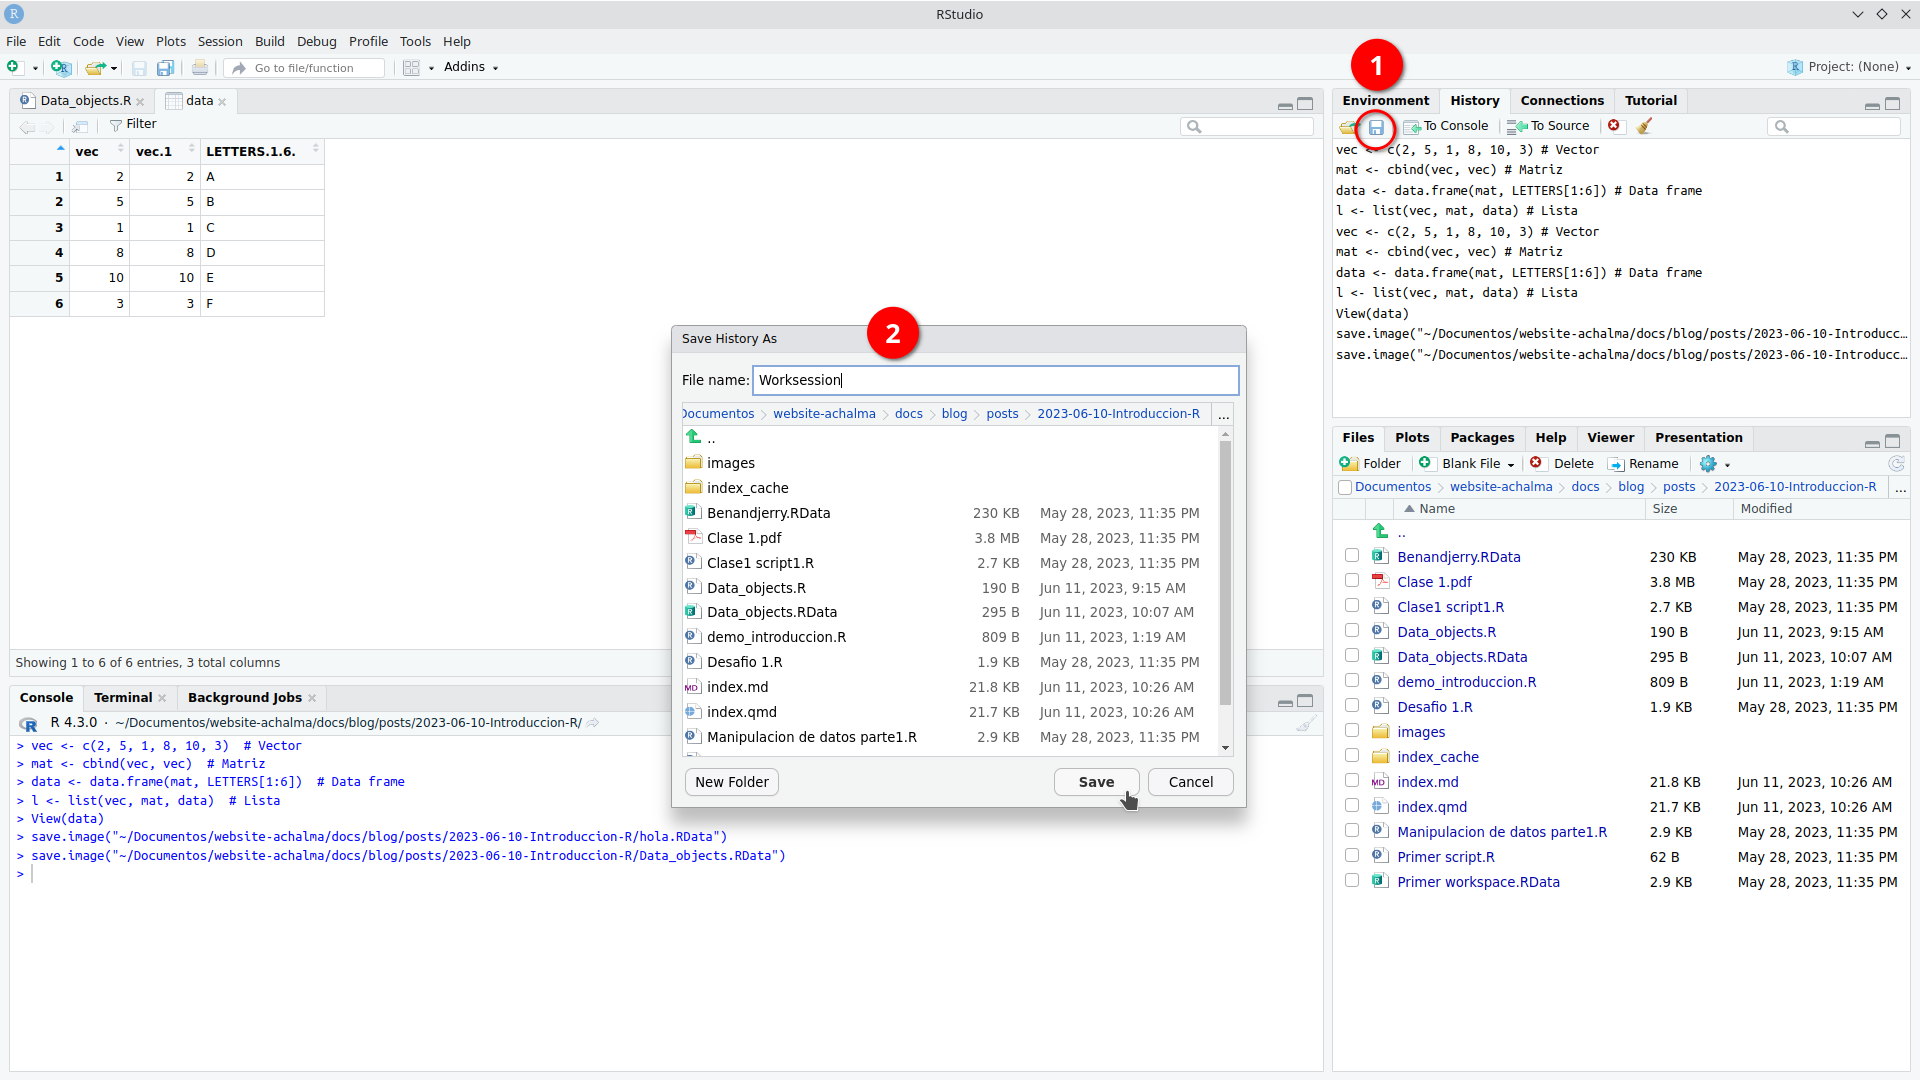
\includegraphics{images/Screenshot_20230611_102856.png}

\hypertarget{reutilizaciuxf3n-del-historial-de-comandos}{%
\subsubsection{Reutilización del historial de
comandos}\label{reutilizaciuxf3n-del-historial-de-comandos}}

El historial se guarda en un archivo llamado \texttt{.Rhistory}. Puedes
reutilizar todo el historial de comandos haciendo clic en el archivo
\texttt{.Rhistory} o con el nombre asignado. Luego, puedes copiarlos y
pegarlos en tu archivo de script actual.

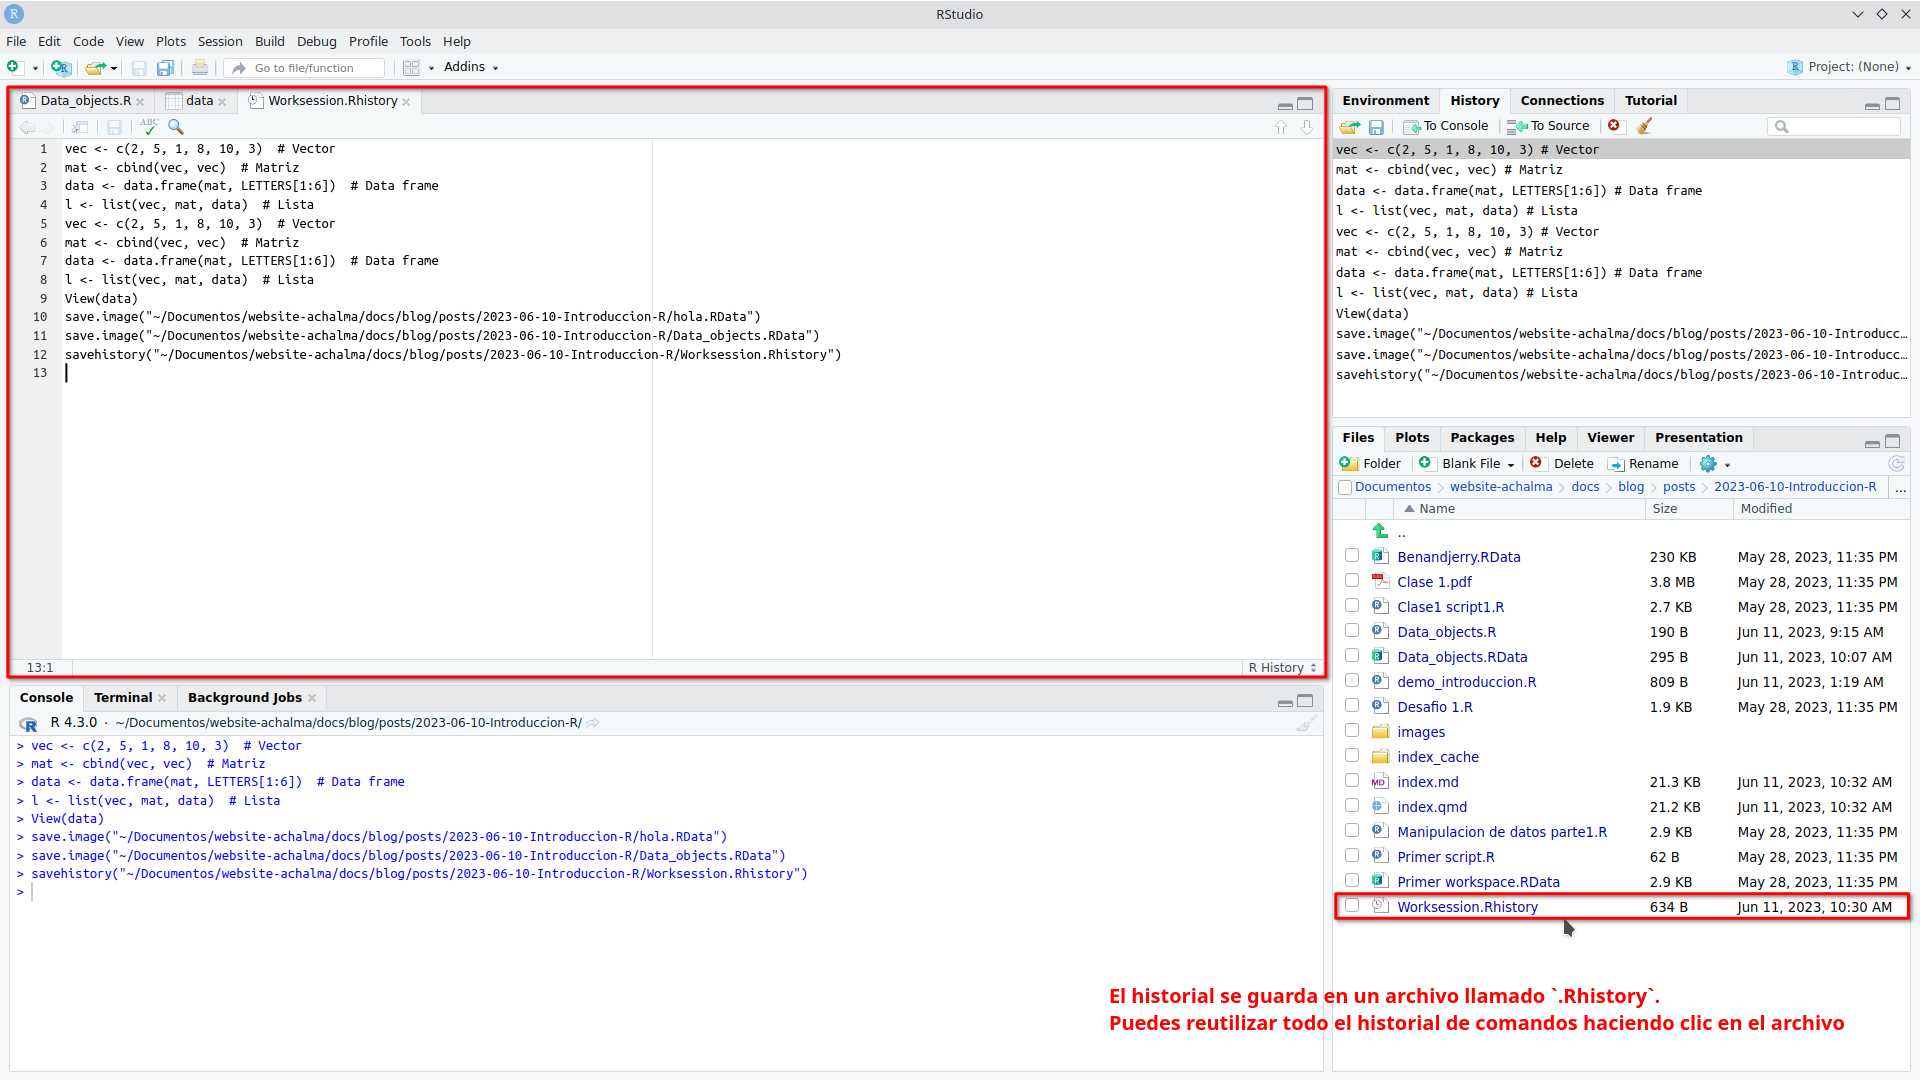
\includegraphics{images/Screenshot_20230611_103319.png}

Inserta un código de línea seleccionado de \texttt{.Rhistory} en un
archivo de script nuevo.

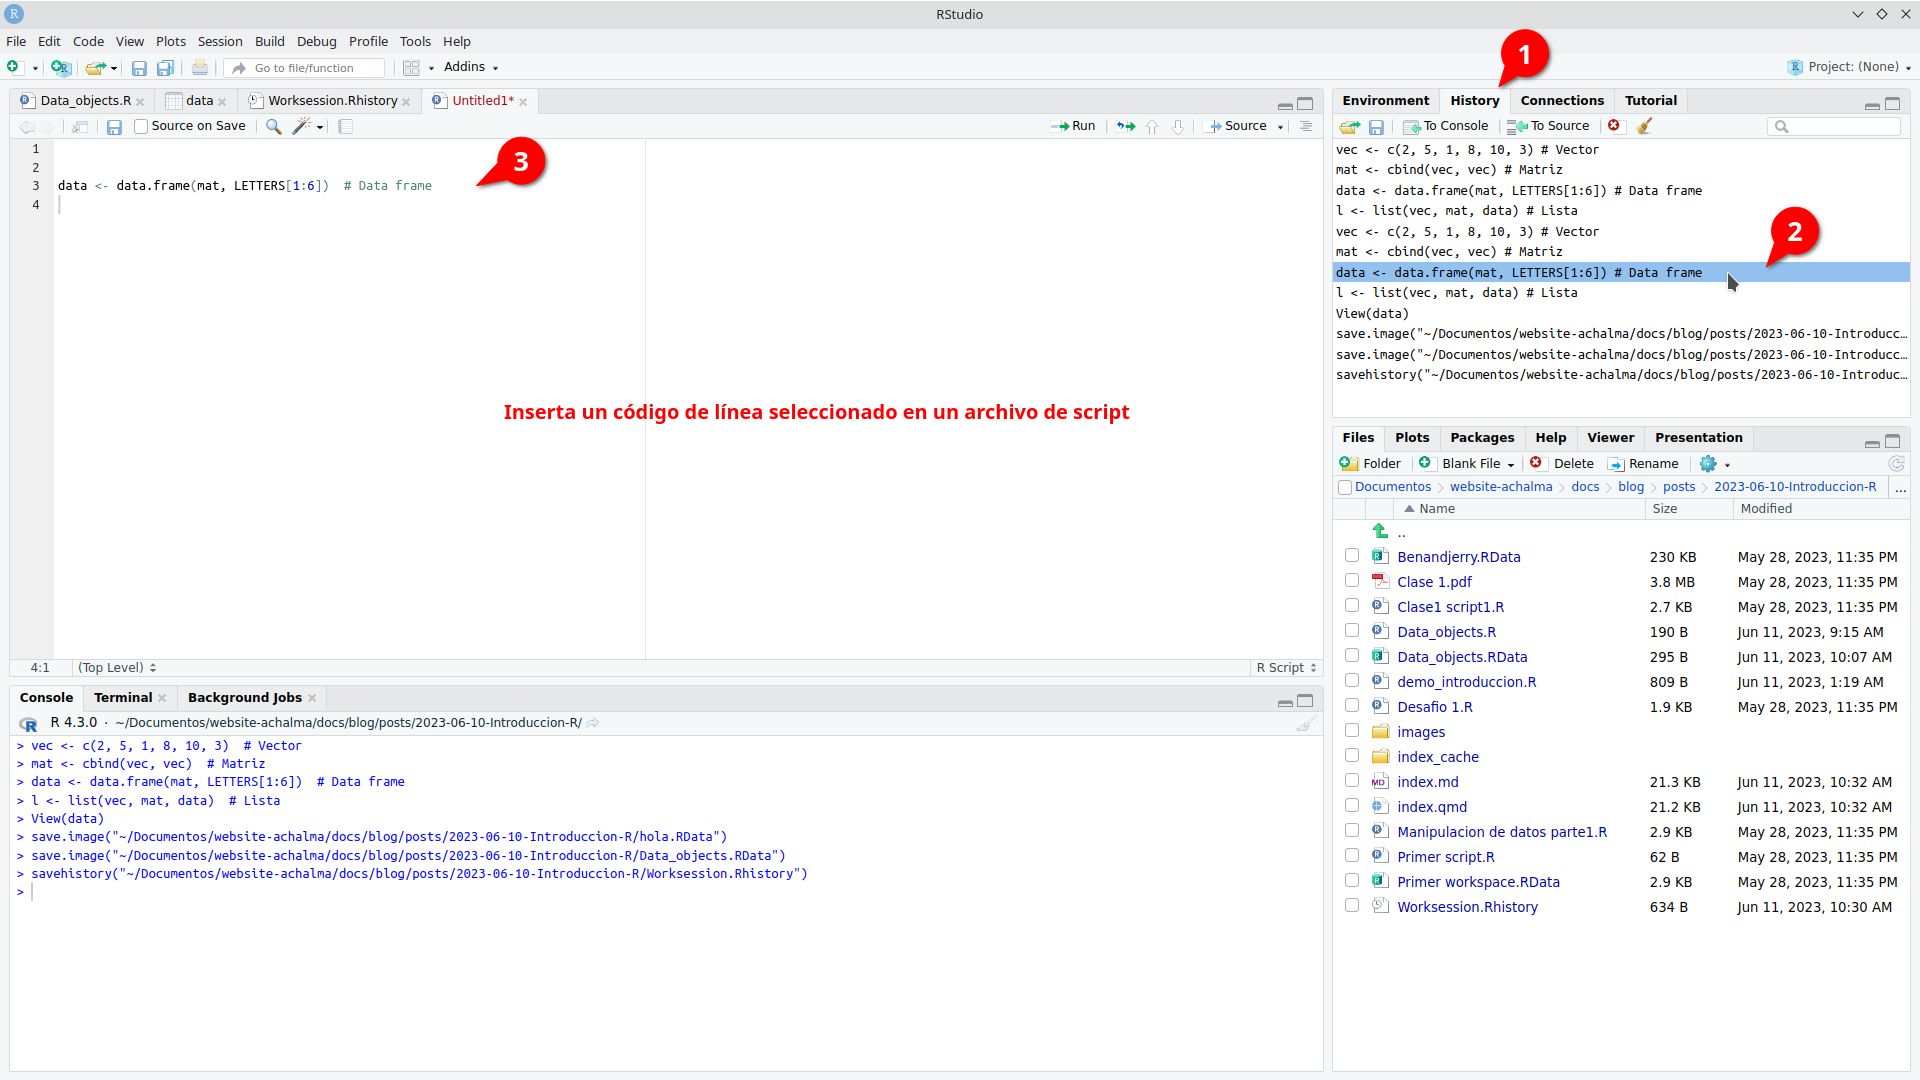
\includegraphics{images/Screenshot_20230611_103755.png}

\begin{quote}
¡Explora y aprovecha al máximo el espacio de trabajo y el historial en
RStudio para mejorar tu flujo de trabajo y aprovechar al máximo tus
comandos y objetos de datos!
\end{quote}


\printbibliography


\end{document}
